\documentclass[landscape]{article}

\usepackage[utf8]{inputenc}
\usepackage[english]{babel}

\usepackage{amsmath,amsfonts,amssymb}
\usepackage{fullpage}
\usepackage{verbatim}

\usepackage[margin=10mm, top=5mm, bottom=5mm]{geometry}

\usepackage{tikz,pgfplots}

\pgfplotsset{
  width=240mm,height=180mm,
  major grid style={thin,dotted,color=black!50},
  minor grid style={thin,dotted,color=black!50},
  grid,
  every axis/.append style={
    line width=0.5pt,
    tick style={
      line cap=round,
      thin,
      major tick length=4pt,
      minor tick length=2pt,
    },
  },
  legend cell align=left,
  legend pos=north west,
  compat=1.9
}

%%%%%%%%%%%%%%%%%%%%%%%%%%%%%%%%%%%%%%%%%%%%%%%%%%%%%%%%%%%%%%%%%%%%%%%%%%%%%%%%

\begin{document}

% IMPORT-DATA ResultsQS ResultsQS_muc.txt

%%%%%%%%%%%%%%%%%%%%%%%%%%%%%%%%%%%%%%%%%%%%%%%%%%%%%%%%%%%%%%%%%%%%%%%%%%%%%%%%

\begin{center}

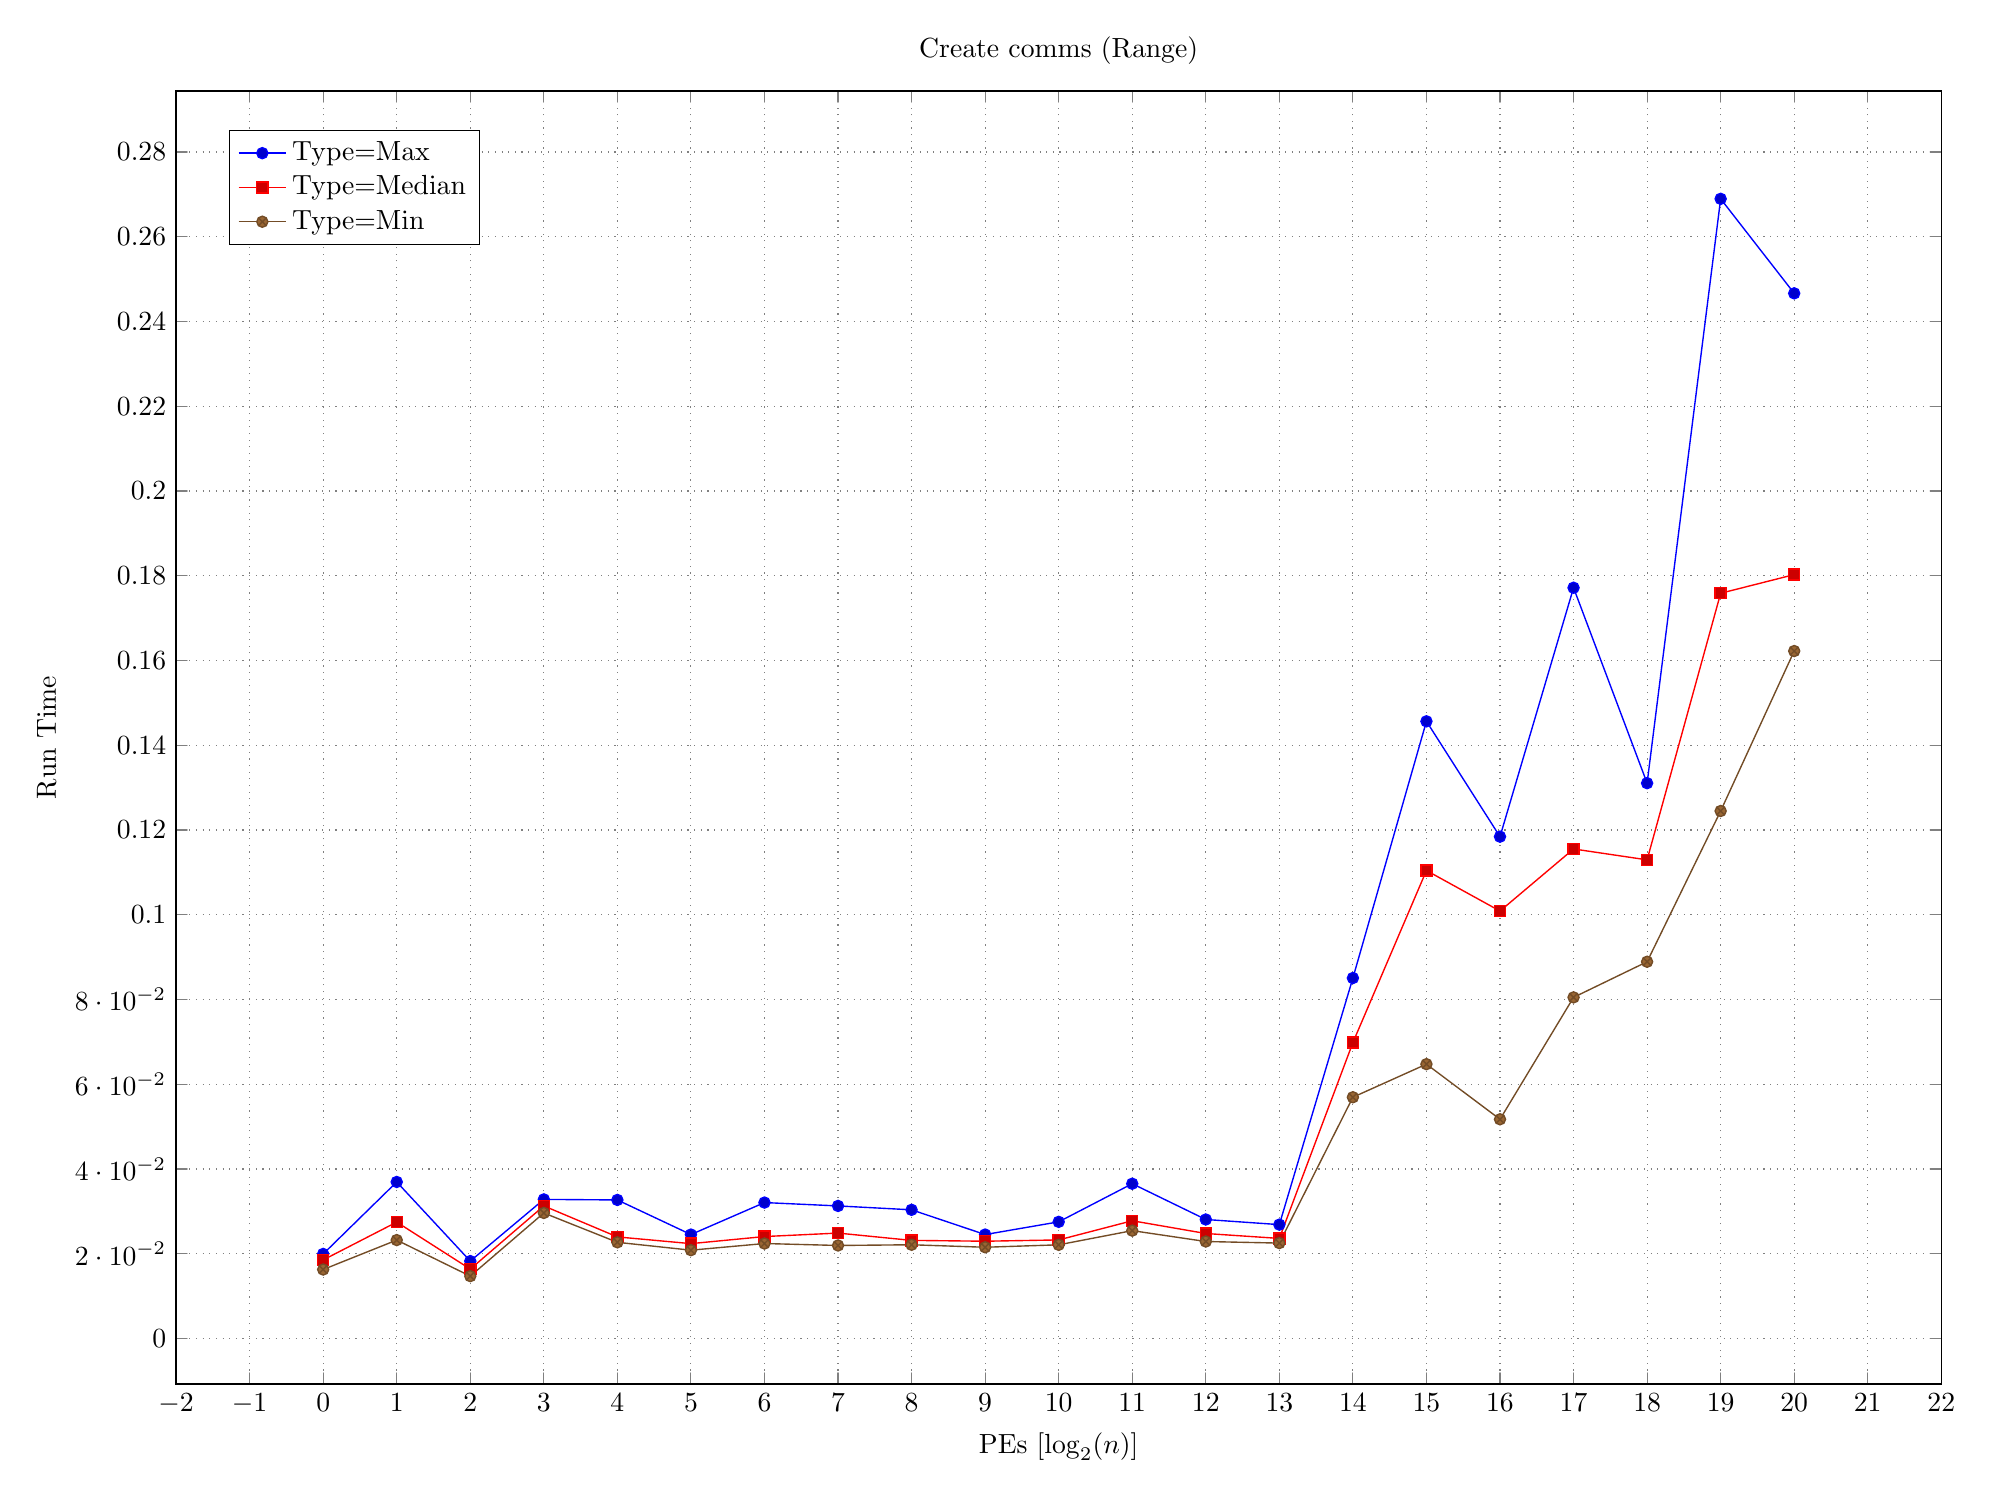
\begin{tikzpicture}
\begin{axis}[
title={Create comms (Range)},
xlabel={PEs [$\log_2(n)$]},
ylabel={Run Time},
]   
%% MULTIPLOT(Type) SELECT size, collective, LOG(2,elements) AS x, Time as y, MULTIPLOT FROM (    
%% SELECT elements, size, MEDIAN(create_comms) as Time, 'Median' as Type, collective
%% FROM ResultsQS
%% GROUP BY collective, size, elements
%% UNION ALL
%% SELECT elements, size, MIN(create_comms) as Time, 'Min' as Type, collective
%% FROM ResultsQS
%% GROUP BY collective, size, elements
%% UNION ALL    
%% SELECT elements, size, MAX(create_comms) as Time, 'Max' as Type, collective
%% FROM ResultsQS
%% GROUP BY collective, size, elements
%% ) a
%% WHERE collective="mpi" AND size=POWER(2,11)
%% GROUP BY MULTIPLOT, x  ORDER BY MULTIPLOT, x
\addplot coordinates { (0.0,0.0199507) (1.0,0.0369374) (2.0,0.0182624) (3.0,0.0328243) (4.0,0.0326949) (5.0,0.0245276) (6.0,0.0320764) (7.0,0.0312827) (8.0,0.0303653) (9.0,0.0245264) (10.0,0.0275252) (11.0,0.0365265) (12.0,0.0280814) (13.0,0.02687) (14.0,0.0850645) (15.0,0.145648) (16.0,0.118424) (17.0,0.177174) (18.0,0.13105) (19.0,0.268956) (20.0,0.246648) };
\addlegendentry{Type=Max};
\addplot coordinates { (0.0,0.0185403) (1.0,0.0274676) (2.0,0.0163795) (3.0,0.0312834) (4.0,0.023969) (5.0,0.022385) (6.0,0.0240554) (7.0,0.0248753) (8.0,0.0231484) (9.0,0.0229543) (10.0,0.0232588) (11.0,0.0277824) (12.0,0.0247744) (13.0,0.0236128) (14.0,0.0698361) (15.0,0.110434) (16.0,0.100875) (17.0,0.115524) (18.0,0.112954) (19.0,0.175868) (20.0,0.180269) };
\addlegendentry{Type=Median};
\addplot coordinates { (0.0,0.0162736) (1.0,0.0232232) (2.0,0.0147127) (3.0,0.0296221) (4.0,0.0226929) (5.0,0.0208385) (6.0,0.0224104) (7.0,0.0219504) (8.0,0.0221163) (9.0,0.0215301) (10.0,0.0221049) (11.0,0.0254506) (12.0,0.0228833) (13.0,0.0225116) (14.0,0.0569339) (15.0,0.0647406) (16.0,0.0517288) (17.0,0.0805002) (18.0,0.0889086) (19.0,0.124483) (20.0,0.162234) };
\addlegendentry{Type=Min};

\end{axis}
\end{tikzpicture}
\newpage

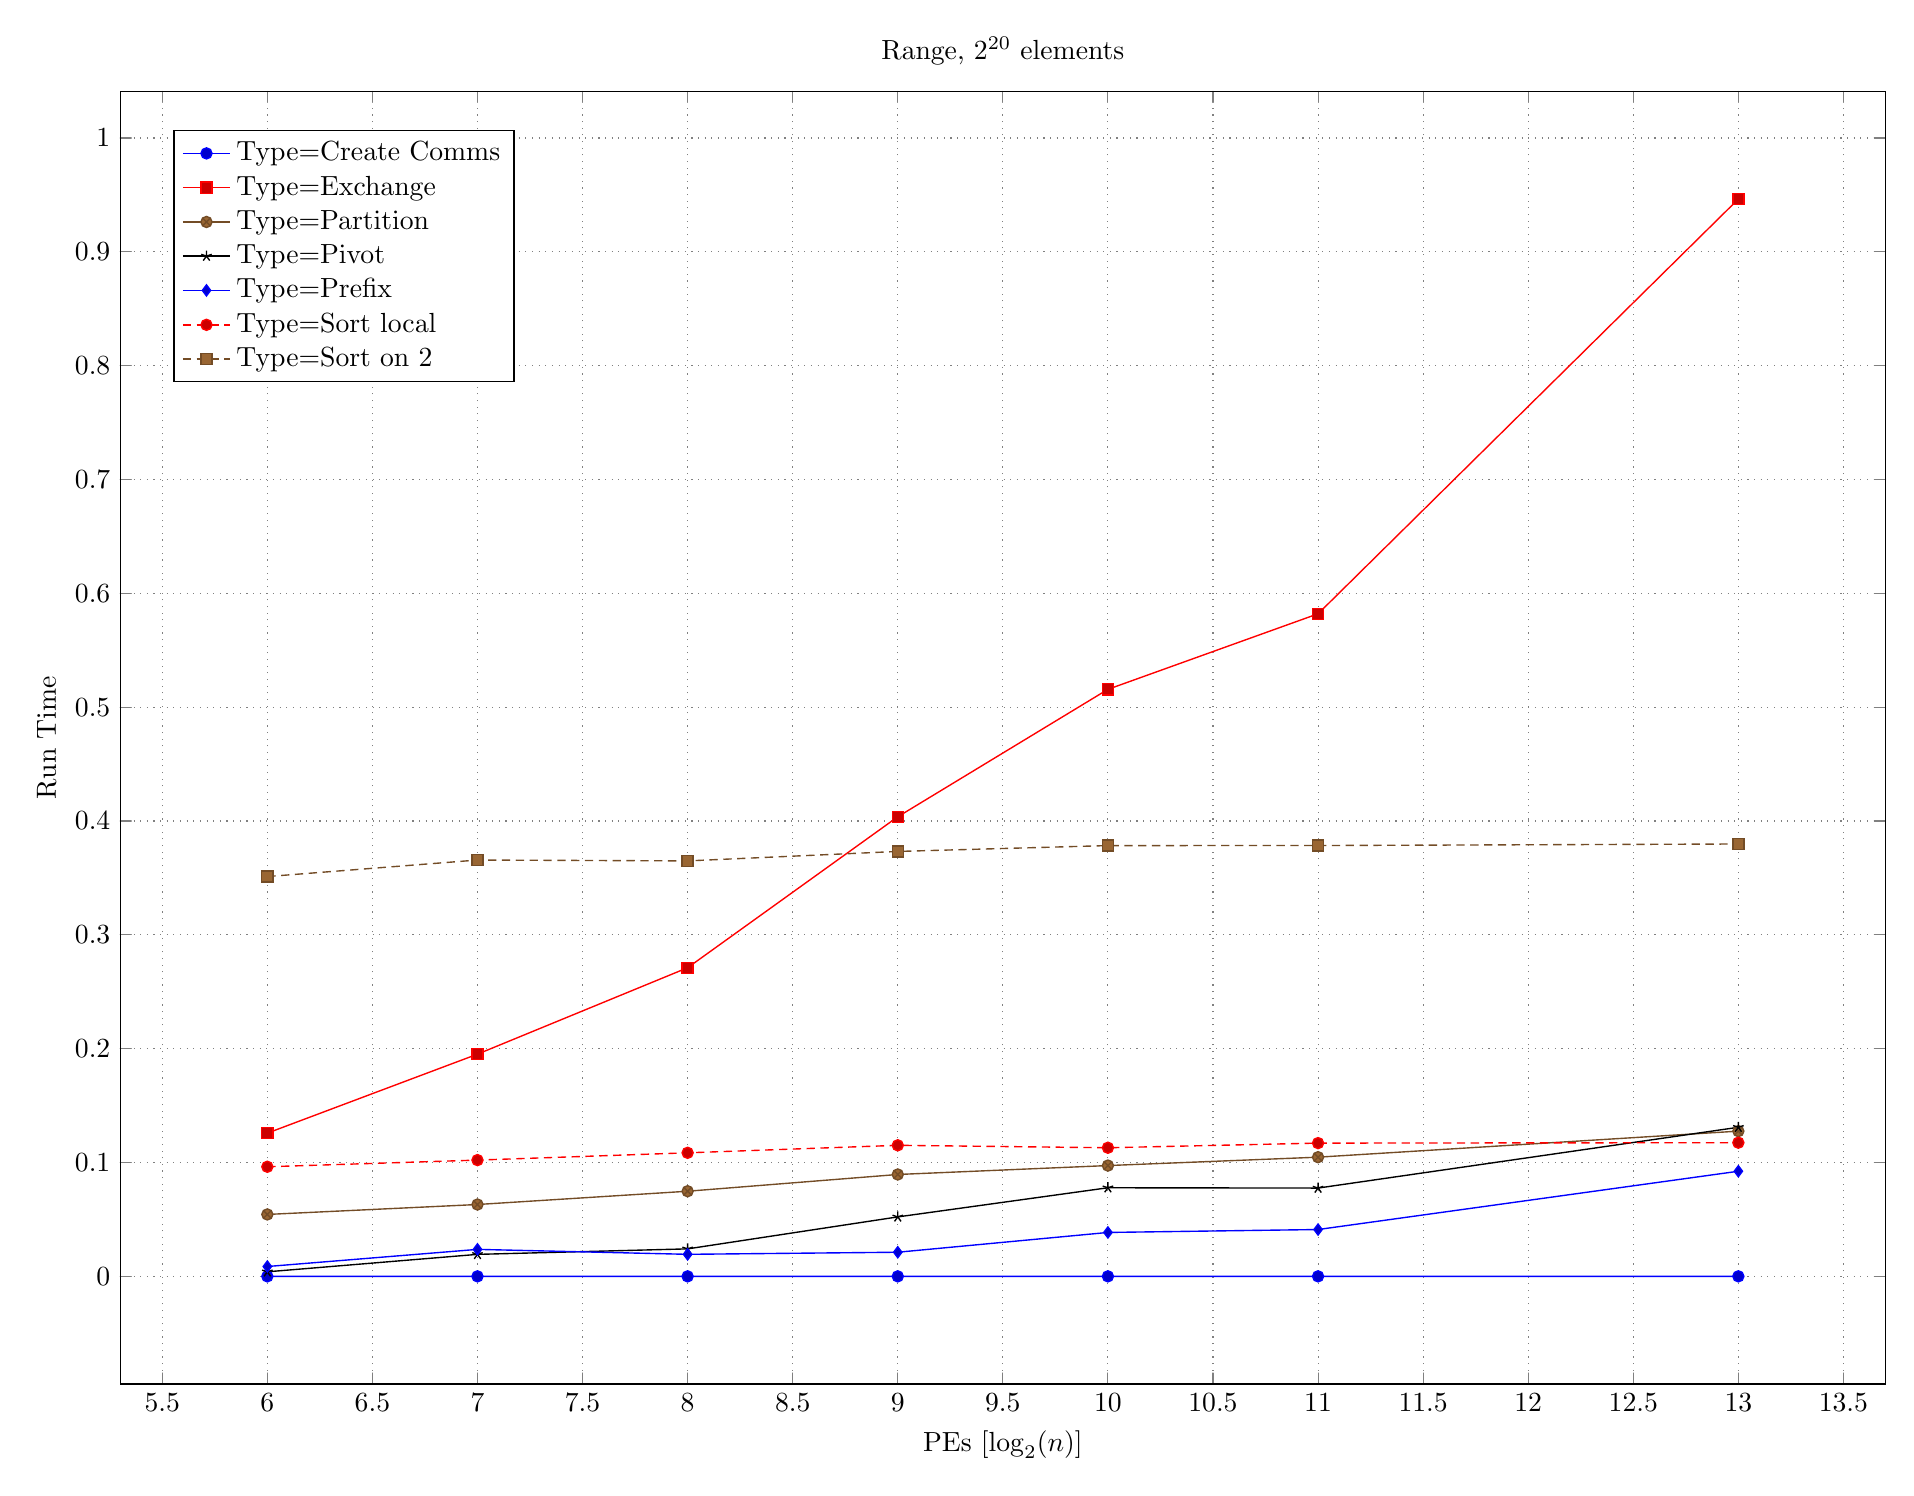
\begin{tikzpicture}
  \begin{axis}[
    title={Range, $2^{20}$ elements},
    xlabel={PEs [$\log_2(n)$]},
    ylabel={Run Time},
    ]   
	%% MULTIPLOT(Type) SELECT elements, collective, LOG(2,size) AS x, Time as y, MULTIPLOT FROM (    
	%% SELECT elements, size, MEDIAN(pivot) as Time, 'Pivot' as Type, collective
	%% FROM ResultsQS
	%% GROUP BY collective, size, elements
	%% UNION ALL
	%% SELECT elements, size, MEDIAN(partition) as Time, 'Partition' as Type, collective
	%% FROM ResultsQS
	%% GROUP BY collective, size, elements
	%% UNION ALL
	%% SELECT elements, size, MEDIAN(calculate) as Time, 'Prefix' as Type, collective
	%% FROM ResultsQS
	%% GROUP BY collective, size, elements
	%% UNION ALL
	%% SELECT elements, size, MEDIAN(exchange) as Time, 'Exchange' as Type, collective
	%% FROM ResultsQS
	%% GROUP BY collective, size, elements
	%% UNION ALL
	%% SELECT elements, size, MEDIAN(create_comms) as Time, 'Create Comms' as Type, collective
	%% FROM ResultsQS
	%% GROUP BY collective, size, elements
	%% UNION ALL
	%% SELECT elements, size, MEDIAN(sort_two) as Time, 'Sort on 2' as Type, collective
	%% FROM ResultsQS
	%% GROUP BY collective, size, elements
	%% UNION ALL
	%% SELECT elements, size, MEDIAN(sort_local) as Time, 'Sort local' as Type, collective
	%% FROM ResultsQS
	%% GROUP BY collective, size, elements
	%% ) a
	%% WHERE collective="range" AND elements=POWER(2,20)
	%% GROUP BY MULTIPLOT, x  ORDER BY MULTIPLOT, x
 \addplot coordinates { (6.0,4.42658e-06) (7.0,5.72578e-06) (8.0,6.71577e-06) (9.0,8.88109e-06) (10.0,1.61929e-05) (11.0,2.03271e-05) (13.0,2.56645e-05) };
 \addlegendentry{Type=Create Comms};
 \addplot coordinates { (6.0,0.125829) (7.0,0.195211) (8.0,0.271121) (9.0,0.403734) (10.0,0.51569) (11.0,0.582063) (13.0,0.946399) };
 \addlegendentry{Type=Exchange};
 \addplot coordinates { (6.0,0.0544023) (7.0,0.0631221) (8.0,0.0747817) (9.0,0.0895008) (10.0,0.0973363) (11.0,0.1047) (13.0,0.127574) };
 \addlegendentry{Type=Partition};
 \addplot coordinates { (6.0,0.0040016) (7.0,0.0193228) (8.0,0.0241468) (9.0,0.052234) (10.0,0.0778279) (11.0,0.0775652) (13.0,0.13096) };
 \addlegendentry{Type=Pivot};
 \addplot coordinates { (6.0,0.00864934) (7.0,0.0237042) (8.0,0.0193636) (9.0,0.0211961) (10.0,0.0385763) (11.0,0.0411422) (13.0,0.0923424) };
 \addlegendentry{Type=Prefix};
 \addplot coordinates { (6.0,0.0962813) (7.0,0.102136) (8.0,0.108535) (9.0,0.115121) (10.0,0.112986) (11.0,0.117063) (13.0,0.117437) };
 \addlegendentry{Type=Sort local};
 \addplot coordinates { (6.0,0.351205) (7.0,0.365738) (8.0,0.364976) (9.0,0.373289) (10.0,0.378437) (11.0,0.37848) (13.0,0.379827) };
 \addlegendentry{Type=Sort on 2};


  \end{axis}
\end{tikzpicture}
\newpage

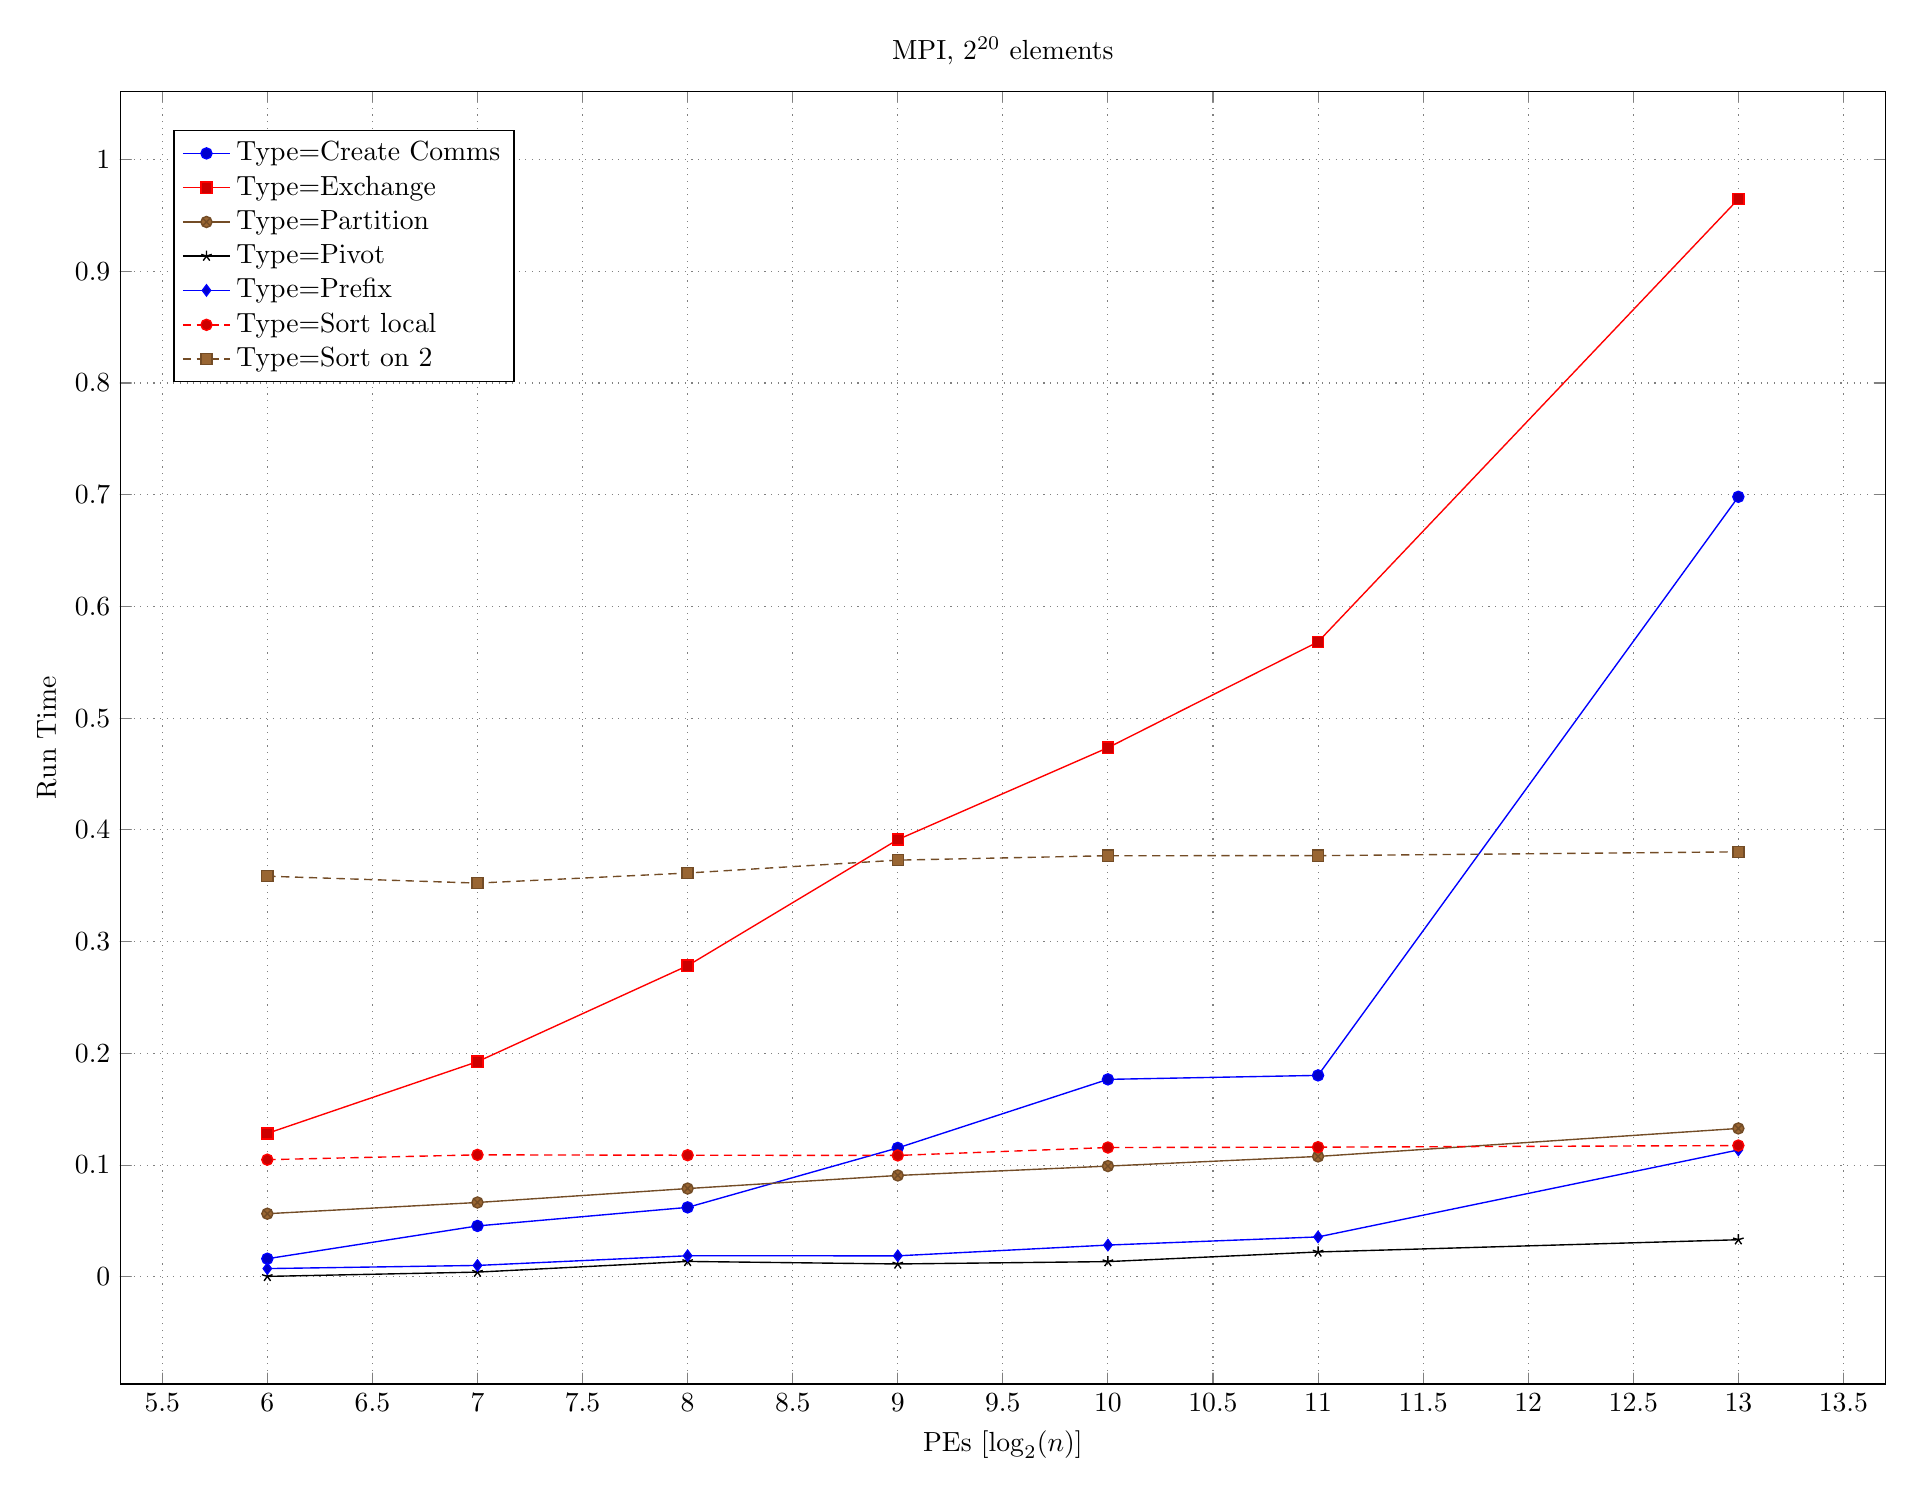
\begin{tikzpicture}
  \begin{axis}[
    title={MPI, $2^{20}$ elements},
    xlabel={PEs [$\log_2(n)$]},
    ylabel={Run Time},
    ]   
	%% MULTIPLOT(Type) SELECT elements, collective, LOG(2,size) AS x, Time as y, MULTIPLOT FROM (    
	%% SELECT elements, size, MEDIAN(pivot) as Time, 'Pivot' as Type, collective
	%% FROM ResultsQS
	%% GROUP BY collective, size, elements
	%% UNION ALL
	%% SELECT elements, size, MEDIAN(partition) as Time, 'Partition' as Type, collective
	%% FROM ResultsQS
	%% GROUP BY collective, size, elements
	%% UNION ALL
	%% SELECT elements, size, MEDIAN(calculate) as Time, 'Prefix' as Type, collective
	%% FROM ResultsQS
	%% GROUP BY collective, size, elements
	%% UNION ALL
	%% SELECT elements, size, MEDIAN(exchange) as Time, 'Exchange' as Type, collective
	%% FROM ResultsQS
	%% GROUP BY collective, size, elements
	%% UNION ALL
	%% SELECT elements, size, MEDIAN(create_comms) as Time, 'Create Comms' as Type, collective
	%% FROM ResultsQS
	%% GROUP BY collective, size, elements
	%% UNION ALL
	%% SELECT elements, size, MEDIAN(sort_two) as Time, 'Sort on 2' as Type, collective
	%% FROM ResultsQS
	%% GROUP BY collective, size, elements
	%% UNION ALL
	%% SELECT elements, size, MEDIAN(sort_local) as Time, 'Sort local' as Type, collective
	%% FROM ResultsQS
	%% GROUP BY collective, size, elements
	%% ) a
	%% WHERE collective="mpi" AND elements=POWER(2,20)
	%% GROUP BY MULTIPLOT, x  ORDER BY MULTIPLOT, x
 \addplot coordinates { (6.0,0.0161887) (7.0,0.0455253) (8.0,0.0621324) (9.0,0.115342) (10.0,0.176707) (11.0,0.180269) (13.0,0.69812) };
 \addlegendentry{Type=Create Comms};
 \addplot coordinates { (6.0,0.12836) (7.0,0.192551) (8.0,0.278452) (9.0,0.39128) (10.0,0.473561) (11.0,0.568296) (13.0,0.964602) };
 \addlegendentry{Type=Exchange};
 \addplot coordinates { (6.0,0.0564817) (7.0,0.0665136) (8.0,0.0789873) (9.0,0.0907094) (10.0,0.0990889) (11.0,0.107729) (13.0,0.13279) };
 \addlegendentry{Type=Partition};
 \addplot coordinates { (6.0,0.000367634) (7.0,0.0041966) (8.0,0.0137521) (9.0,0.0114884) (10.0,0.013606) (11.0,0.0222273) (13.0,0.0331757) };
 \addlegendentry{Type=Pivot};
 \addplot coordinates { (6.0,0.00735342) (7.0,0.010175) (8.0,0.0188407) (9.0,0.0187714) (10.0,0.028407) (11.0,0.0356952) (13.0,0.113538) };
 \addlegendentry{Type=Prefix};
 \addplot coordinates { (6.0,0.104822) (7.0,0.109148) (8.0,0.108821) (9.0,0.108623) (10.0,0.115708) (11.0,0.116034) (13.0,0.11747) };
 \addlegendentry{Type=Sort local};
 \addplot coordinates { (6.0,0.358551) (7.0,0.35237) (8.0,0.361393) (9.0,0.372918) (10.0,0.376887) (11.0,0.376924) (13.0,0.380349) };
 \addlegendentry{Type=Sort on 2};

  \end{axis}
\end{tikzpicture}
\newpage

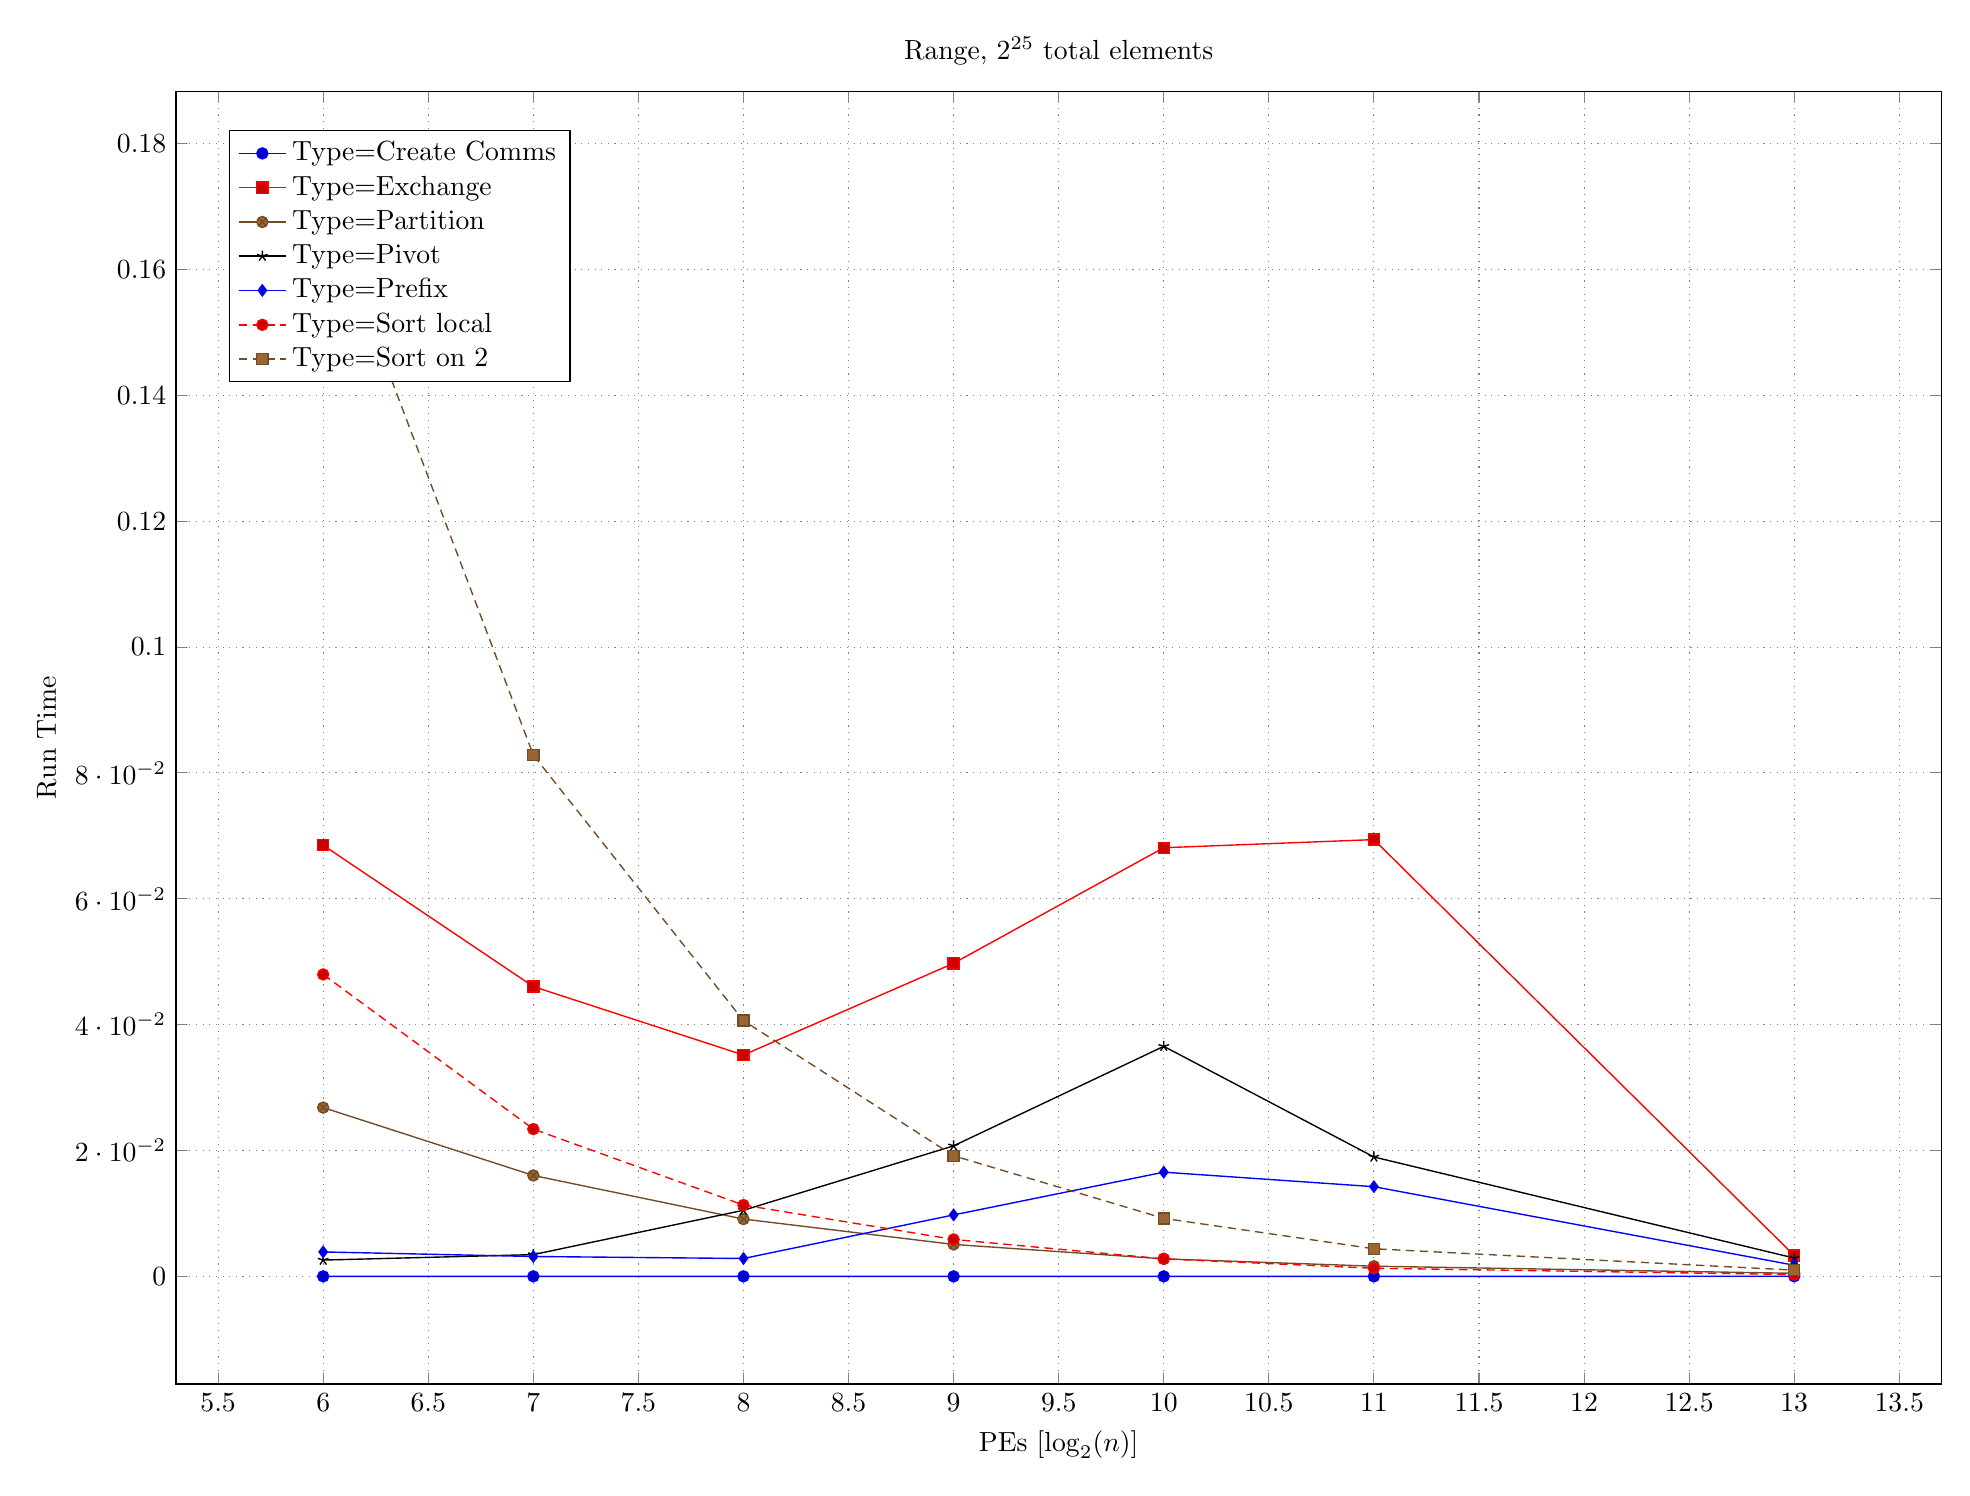
\begin{tikzpicture}
\begin{axis}[
title={Range, $2^{25}$ total elements},
xlabel={PEs [$\log_2(n)$]},
ylabel={Run Time},
]   
%% MULTIPLOT(Type) SELECT elements*size AS total_elements, collective, LOG(2,size) AS x, Time as y, MULTIPLOT FROM (    
%% SELECT elements, size, MEDIAN(pivot) as Time, 'Pivot' as Type, collective
%% FROM ResultsQS
%% GROUP BY collective, size, elements
%% UNION ALL
%% SELECT elements, size, MEDIAN(partition) as Time, 'Partition' as Type, collective
%% FROM ResultsQS
%% GROUP BY collective, size, elements
%% UNION ALL
%% SELECT elements, size, MEDIAN(calculate) as Time, 'Prefix' as Type, collective
%% FROM ResultsQS
%% GROUP BY collective, size, elements
%% UNION ALL
%% SELECT elements, size, MEDIAN(exchange) as Time, 'Exchange' as Type, collective
%% FROM ResultsQS
%% GROUP BY collective, size, elements
%% UNION ALL
%% SELECT elements, size, MEDIAN(create_comms) as Time, 'Create Comms' as Type, collective
%% FROM ResultsQS
%% GROUP BY collective, size, elements
%% UNION ALL
%% SELECT elements, size, MEDIAN(sort_two) as Time, 'Sort on 2' as Type, collective
%% FROM ResultsQS
%% GROUP BY collective, size, elements
%% UNION ALL
%% SELECT elements, size, MEDIAN(sort_local) as Time, 'Sort local' as Type, collective
%% FROM ResultsQS
%% GROUP BY collective, size, elements
%% ) a
%% WHERE collective="range" AND total_elements=POWER(2,25)
%% GROUP BY MULTIPLOT, x  ORDER BY MULTIPLOT, x
\addplot coordinates { (6.0,4.1714e-06) (7.0,4.40795e-06) (8.0,3.14694e-06) (9.0,2.58907e-06) (10.0,2.57604e-06) (11.0,3.28571e-06) (13.0,1.7263e-05) };
\addlegendentry{Type=Create Comms};
\addplot coordinates { (6.0,0.0685147) (7.0,0.0460564) (8.0,0.0351756) (9.0,0.0497534) (10.0,0.068115) (11.0,0.0694044) (13.0,0.00332207) };
\addlegendentry{Type=Exchange};
\addplot coordinates { (6.0,0.0268227) (7.0,0.0160371) (8.0,0.00910693) (9.0,0.00507652) (10.0,0.00278854) (11.0,0.00161797) (13.0,0.000489571) };
\addlegendentry{Type=Partition};
\addplot coordinates { (6.0,0.00259146) (7.0,0.00345934) (8.0,0.0105056) (9.0,0.0207446) (10.0,0.0365562) (11.0,0.0189722) (13.0,0.00291346) };
\addlegendentry{Type=Pivot};
\addplot coordinates { (6.0,0.00388462) (7.0,0.0031613) (8.0,0.00284497) (9.0,0.0097663) (10.0,0.0165582) (11.0,0.0142556) (13.0,0.00177364) };
\addlegendentry{Type=Prefix};
\addplot coordinates { (6.0,0.0479823) (7.0,0.0234079) (8.0,0.0113356) (9.0,0.00587062) (10.0,0.00278145) (11.0,0.00129645) (13.0,0.000294444) };
\addlegendentry{Type=Sort local};
\addplot coordinates { (6.0,0.171191) (7.0,0.0828334) (8.0,0.040639) (9.0,0.0191642) (10.0,0.00922053) (11.0,0.00438891) (13.0,0.000995412) };
\addlegendentry{Type=Sort on 2};


\end{axis}
\end{tikzpicture}
\newpage

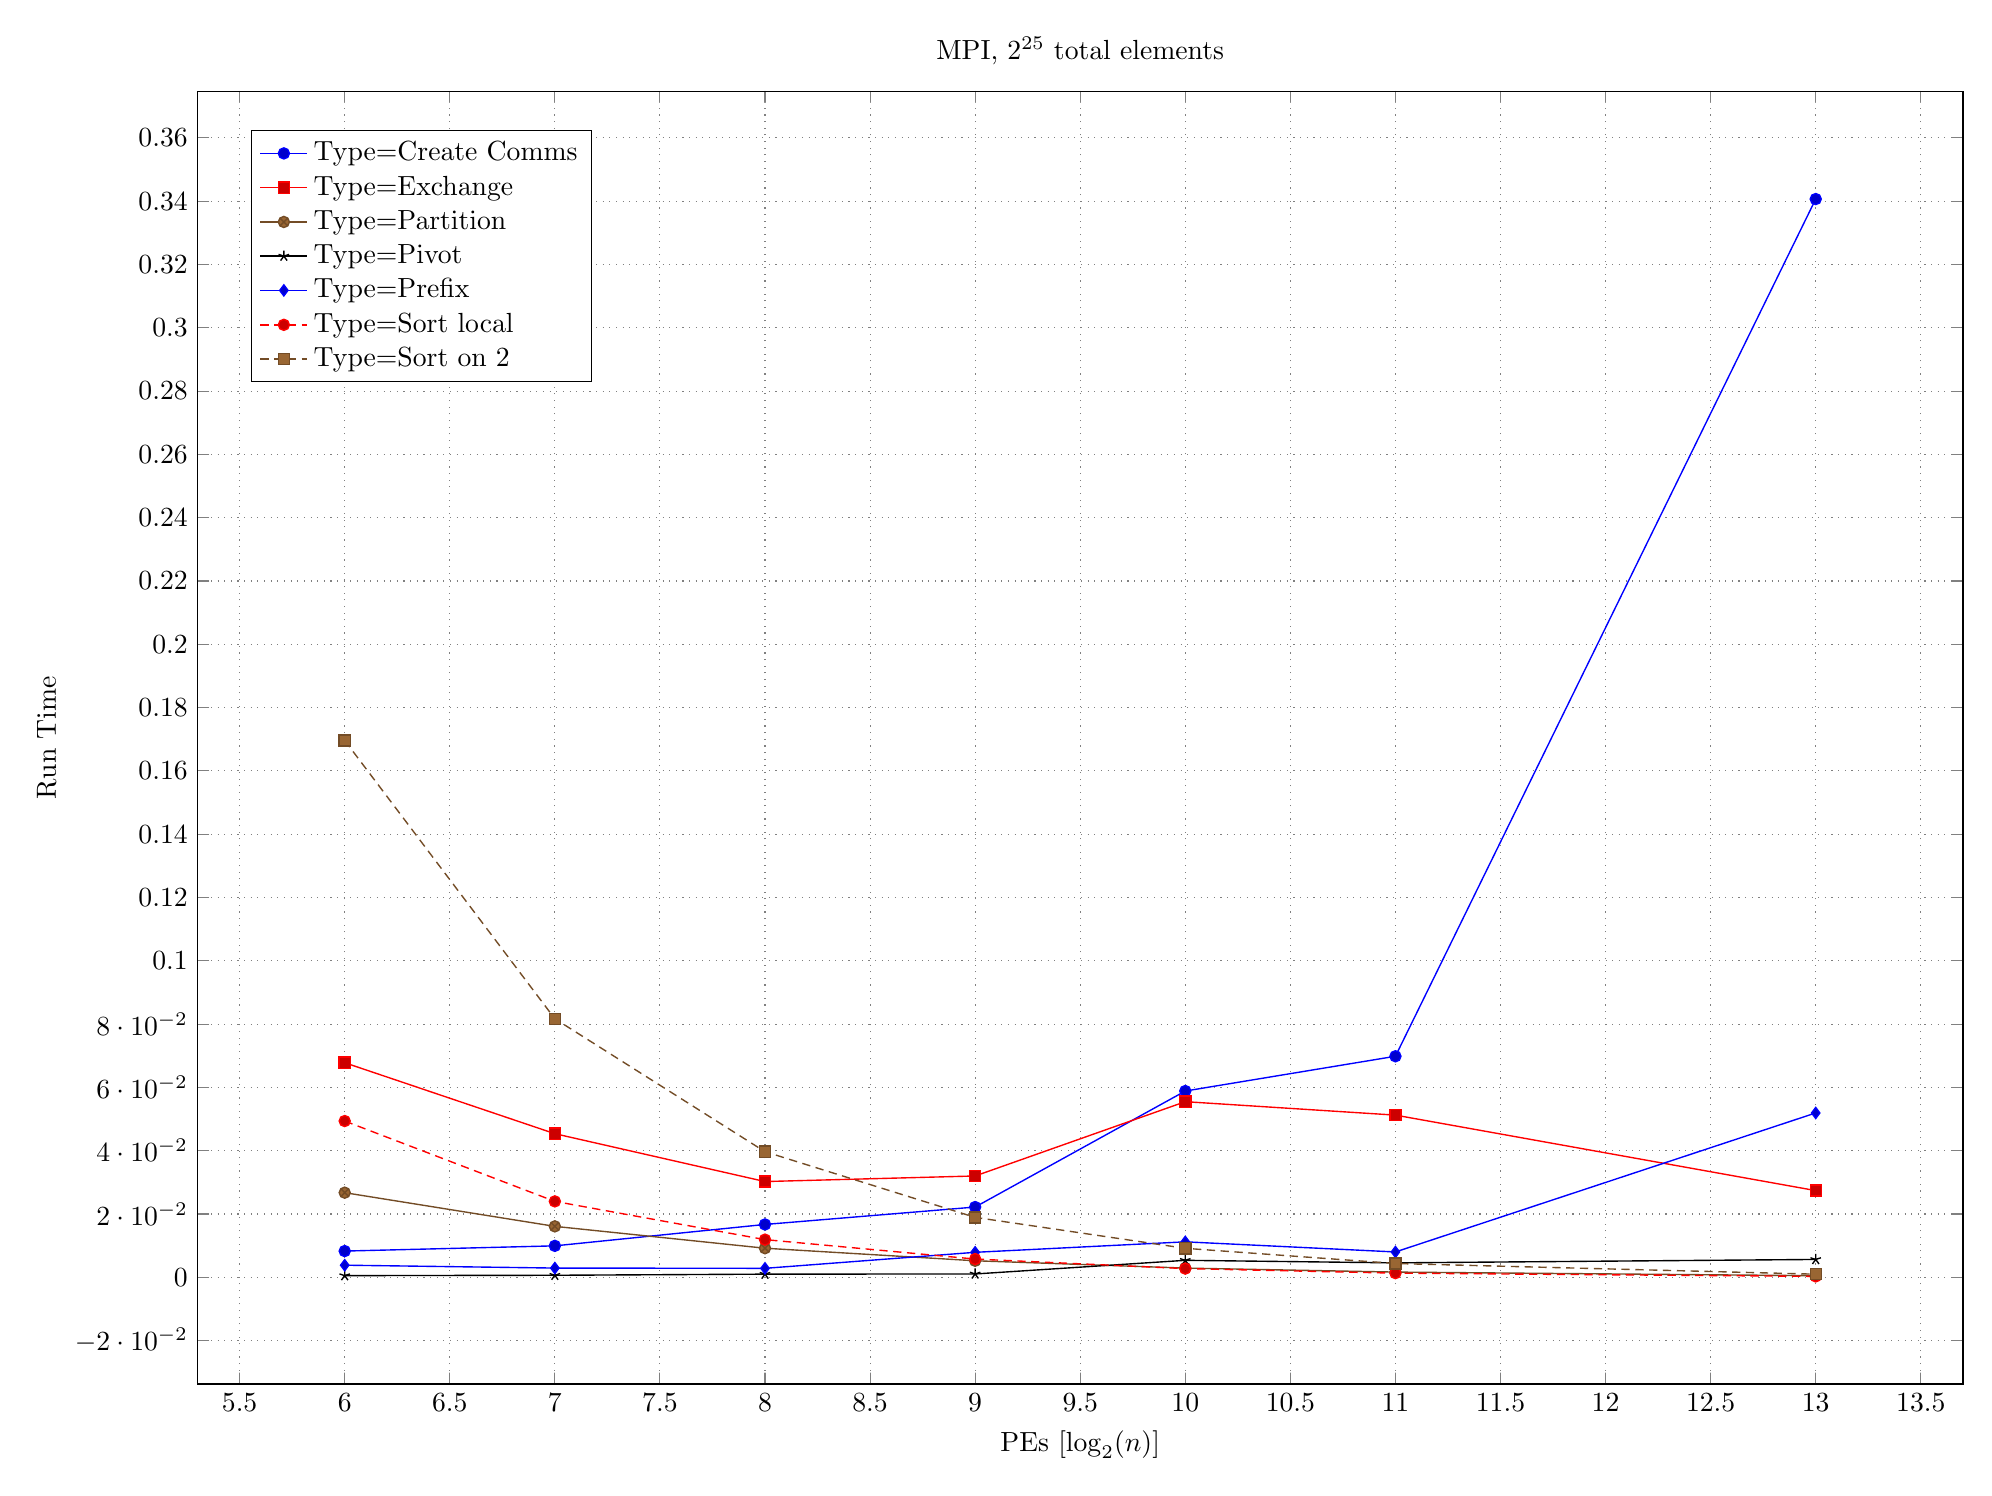
\begin{tikzpicture}
\begin{axis}[
title={MPI, $2^{25}$ total elements},
xlabel={PEs [$\log_2(n)$]},
ylabel={Run Time},
]   
%% MULTIPLOT(Type) SELECT elements*size AS total_elements, collective, LOG(2,size) AS x, Time as y, MULTIPLOT FROM (    
%% SELECT elements, size, MEDIAN(pivot) as Time, 'Pivot' as Type, collective
%% FROM ResultsQS
%% GROUP BY collective, size, elements
%% UNION ALL
%% SELECT elements, size, MEDIAN(partition) as Time, 'Partition' as Type, collective
%% FROM ResultsQS
%% GROUP BY collective, size, elements
%% UNION ALL
%% SELECT elements, size, MEDIAN(calculate) as Time, 'Prefix' as Type, collective
%% FROM ResultsQS
%% GROUP BY collective, size, elements
%% UNION ALL
%% SELECT elements, size, MEDIAN(exchange) as Time, 'Exchange' as Type, collective
%% FROM ResultsQS
%% GROUP BY collective, size, elements
%% UNION ALL
%% SELECT elements, size, MEDIAN(create_comms) as Time, 'Create Comms' as Type, collective
%% FROM ResultsQS
%% GROUP BY collective, size, elements
%% UNION ALL
%% SELECT elements, size, MEDIAN(sort_two) as Time, 'Sort on 2' as Type, collective
%% FROM ResultsQS
%% GROUP BY collective, size, elements
%% UNION ALL
%% SELECT elements, size, MEDIAN(sort_local) as Time, 'Sort local' as Type, collective
%% FROM ResultsQS
%% GROUP BY collective, size, elements
%% ) a
%% WHERE collective="mpi" AND total_elements=POWER(2,25)
%% GROUP BY MULTIPLOT, x  ORDER BY MULTIPLOT, x
\addplot coordinates { (6.0,0.00828855) (7.0,0.00993806) (8.0,0.0166975) (9.0,0.0221982) (10.0,0.0588526) (11.0,0.0698361) (13.0,0.340667) };
\addlegendentry{Type=Create Comms};
\addplot coordinates { (6.0,0.0677958) (7.0,0.0453732) (8.0,0.0302525) (9.0,0.0320138) (10.0,0.0554903) (11.0,0.0512415) (13.0,0.0273953) };
\addlegendentry{Type=Exchange};
\addplot coordinates { (6.0,0.0267397) (7.0,0.0160951) (8.0,0.00918919) (9.0,0.00522509) (10.0,0.00291289) (11.0,0.00164972) (13.0,0.000510117) };
\addlegendentry{Type=Partition};
\addplot coordinates { (6.0,0.000530497) (7.0,0.000643326) (8.0,0.00100119) (9.0,0.00105384) (10.0,0.00536358) (11.0,0.0045649) (13.0,0.00564039) };
\addlegendentry{Type=Pivot};
\addplot coordinates { (6.0,0.00382766) (7.0,0.00292027) (8.0,0.00283575) (9.0,0.00789455) (10.0,0.0112085) (11.0,0.00800985) (13.0,0.0519271) };
\addlegendentry{Type=Prefix};
\addplot coordinates { (6.0,0.0493724) (7.0,0.0239891) (8.0,0.0119069) (9.0,0.00576872) (10.0,0.00275423) (11.0,0.00131462) (13.0,0.00029455) };
\addlegendentry{Type=Sort local};
\addplot coordinates { (6.0,0.169611) (7.0,0.0816812) (8.0,0.0396859) (9.0,0.0189363) (10.0,0.0091597) (11.0,0.00435857) (13.0,0.000987884) };
\addlegendentry{Type=Sort on 2};


\end{axis}
\end{tikzpicture}
\newpage

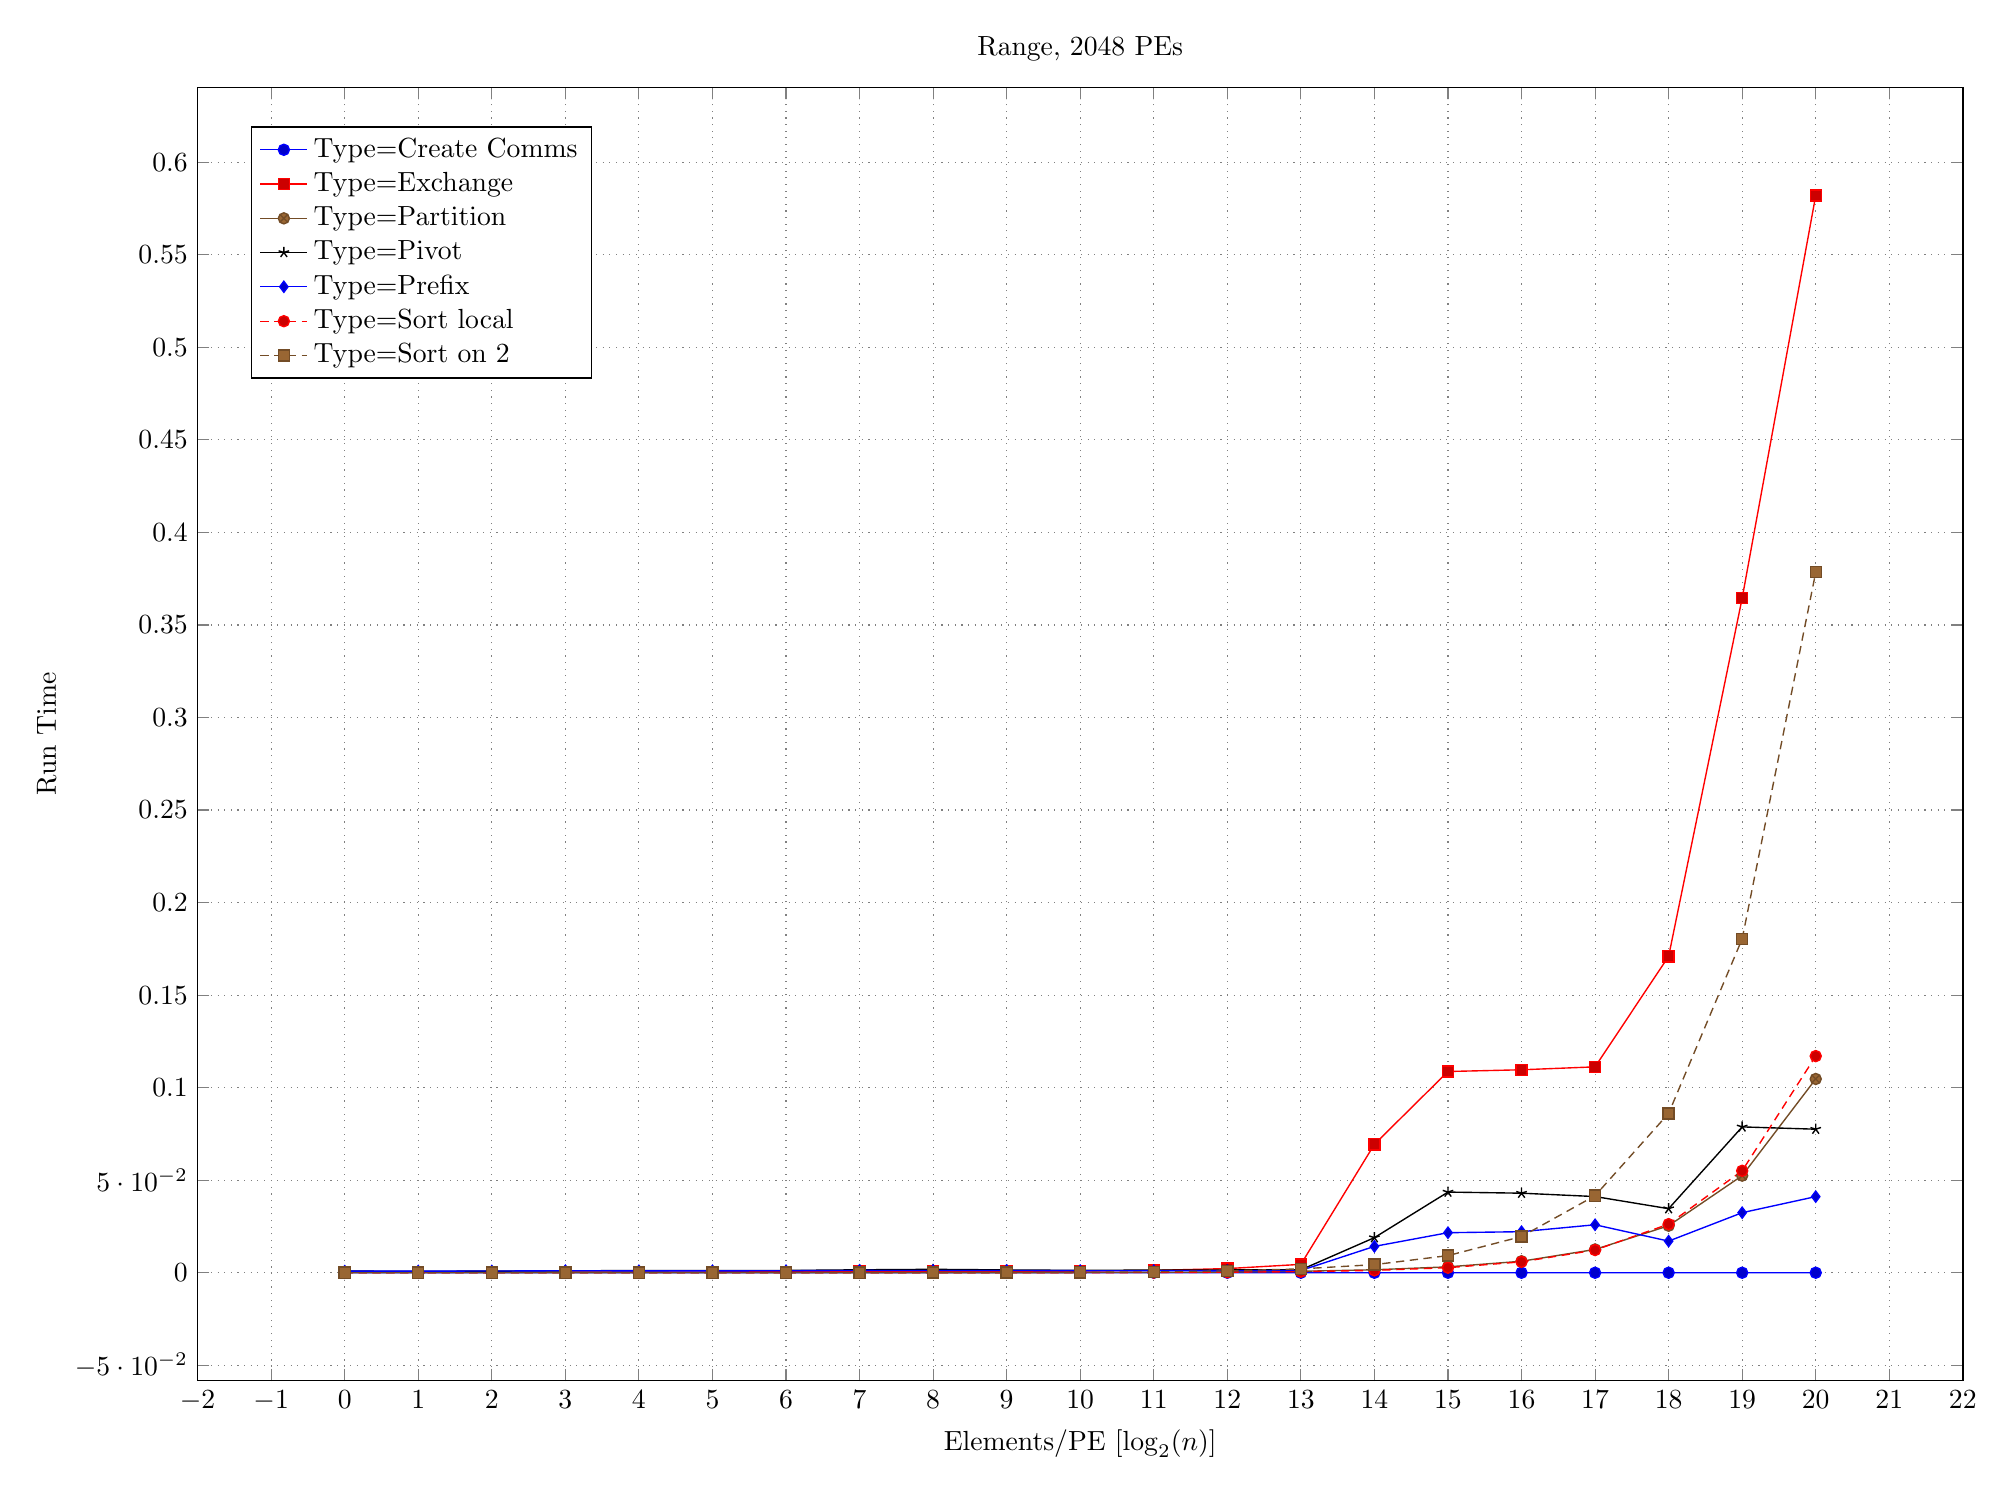
\begin{tikzpicture}
  \begin{axis}[
    title={Range, 2048 PEs},
    xlabel={Elements/PE [$\log_2(n)$]},
    ylabel={Run Time},
    ]   
	%% MULTIPLOT(Type) SELECT size, collective, LOG(2,elements) AS x, Time as y, MULTIPLOT FROM (    
	%% SELECT elements, size, MEDIAN(pivot) as Time, 'Pivot' as Type, collective
	%% FROM ResultsQS
	%% GROUP BY collective, size, elements
	%% UNION ALL
	%% SELECT elements, size, MEDIAN(partition) as Time, 'Partition' as Type, collective
	%% FROM ResultsQS
	%% GROUP BY collective, size, elements
	%% UNION ALL
	%% SELECT elements, size, MEDIAN(calculate) as Time, 'Prefix' as Type, collective
	%% FROM ResultsQS
	%% GROUP BY collective, size, elements
	%% UNION ALL
	%% SELECT elements, size, MEDIAN(exchange) as Time, 'Exchange' as Type, collective
	%% FROM ResultsQS
	%% GROUP BY collective, size, elements
	%% UNION ALL
	%% SELECT elements, size, MEDIAN(create_comms) as Time, 'Create Comms' as Type, collective
	%% FROM ResultsQS
	%% GROUP BY collective, size, elements
	%% UNION ALL
	%% SELECT elements, size, MEDIAN(sort_two) as Time, 'Sort on 2' as Type, collective
	%% FROM ResultsQS
	%% GROUP BY collective, size, elements
	%% UNION ALL
	%% SELECT elements, size, MEDIAN(sort_local) as Time, 'Sort local' as Type, collective
	%% FROM ResultsQS
	%% GROUP BY collective, size, elements
	%% ) a
	%% WHERE collective="range" AND size=2048
	%% GROUP BY MULTIPLOT, x  ORDER BY MULTIPLOT, x
 \addplot coordinates { (0.0,6.85454e-06) (1.0,2.19699e-06) (2.0,2.37115e-06) (3.0,2.2687e-06) (4.0,2.46148e-06) (5.0,8.69948e-06) (6.0,3.9665e-06) (7.0,5.24893e-06) (8.0,4.96581e-06) (9.0,7.58004e-06) (10.0,4.96954e-06) (11.0,2.57511e-06) (12.0,2.50805e-06) (13.0,3.04356e-06) (14.0,3.28571e-06) (15.0,7.11345e-06) (16.0,9.36911e-06) (17.0,1.24518e-05) (18.0,1.79652e-05) (19.0,2.14521e-05) (20.0,2.03271e-05) };
 \addlegendentry{Type=Create Comms};
 \addplot coordinates { (0.0,0.000399966) (1.0,0.000383573) (2.0,0.000246479) (3.0,0.000308109) (4.0,0.00032754) (5.0,0.000450401) (6.0,0.000545178) (7.0,0.000614658) (8.0,0.000676731) (9.0,0.000705041) (10.0,0.000905903) (11.0,0.00127408) (12.0,0.00225279) (13.0,0.00453922) (14.0,0.0694044) (15.0,0.10874) (16.0,0.109668) (17.0,0.111248) (18.0,0.170965) (19.0,0.364505) (20.0,0.582063) };
 \addlegendentry{Type=Exchange};
 \addplot coordinates { (0.0,4.42937e-06) (1.0,4.35301e-06) (2.0,2.18395e-06) (3.0,5.06639e-06) (4.0,1.39418e-05) (5.0,1.37836e-05) (6.0,2.00523e-05) (7.0,2.53367e-05) (8.0,3.66652e-05) (9.0,5.85941e-05) (10.0,0.000109999) (11.0,0.000209068) (12.0,0.000410219) (13.0,0.000798189) (14.0,0.00161797) (15.0,0.00319652) (16.0,0.00621936) (17.0,0.0126067) (18.0,0.0254069) (19.0,0.0524749) (20.0,0.1047) };
 \addlegendentry{Type=Partition};
 \addplot coordinates { (0.0,0.000861186) (1.0,0.000831986) (2.0,0.000865711) (3.0,0.00107465) (4.0,0.00116785) (5.0,0.00122781) (6.0,0.00124143) (7.0,0.00160377) (8.0,0.00185469) (9.0,0.00153917) (10.0,0.00128842) (11.0,0.00146047) (12.0,0.0015287) (13.0,0.0015766) (14.0,0.0189722) (15.0,0.0435926) (16.0,0.0429916) (17.0,0.0411711) (18.0,0.0346173) (19.0,0.0788041) (20.0,0.0775652) };
 \addlegendentry{Type=Pivot};
 \addplot coordinates { (0.0,0.000845094) (1.0,0.000904285) (2.0,0.000932194) (3.0,0.00110154) (4.0,0.00103115) (5.0,0.00103053) (6.0,0.00108406) (7.0,0.0012646) (8.0,0.00121335) (9.0,0.00123831) (10.0,0.00111046) (11.0,0.00109206) (12.0,0.00104279) (13.0,0.00122618) (14.0,0.0142556) (15.0,0.0216445) (16.0,0.0221911) (17.0,0.0259371) (18.0,0.0170997) (19.0,0.0324574) (20.0,0.0411422) };
 \addlegendentry{Type=Prefix};
 \addplot coordinates { (0.0,2.6077e-07) (1.0,3.36208e-07) (2.0,3.95812e-07) (3.0,5.15021e-07) (4.0,6.79866e-07) (5.0,1.48081e-06) (6.0,2.79118e-06) (7.0,6.0061e-06) (8.0,1.30124e-05) (9.0,2.85376e-05) (10.0,6.10268e-05) (11.0,0.000133496) (12.0,0.000286355) (13.0,0.000611027) (14.0,0.00129645) (15.0,0.00274039) (16.0,0.00590427) (17.0,0.0122687) (18.0,0.0262707) (19.0,0.0550947) (20.0,0.117063) };
 \addlegendentry{Type=Sort local};
 \addplot coordinates { (0.0,3.65907e-05) (1.0,2.36807e-05) (2.0,2.50609e-05) (3.0,2.74396e-05) (4.0,2.96896e-05) (5.0,3.06973e-05) (6.0,3.57898e-05) (7.0,4.87287e-05) (8.0,6.73122e-05) (9.0,0.000114465) (10.0,0.000236013) (11.0,0.000468537) (12.0,0.000992907) (13.0,0.00210693) (14.0,0.00438891) (15.0,0.00926743) (16.0,0.0195651) (17.0,0.0416304) (18.0,0.0861062) (19.0,0.180413) (20.0,0.37848) };
 \addlegendentry{Type=Sort on 2};

  \end{axis}
\end{tikzpicture}
\newpage

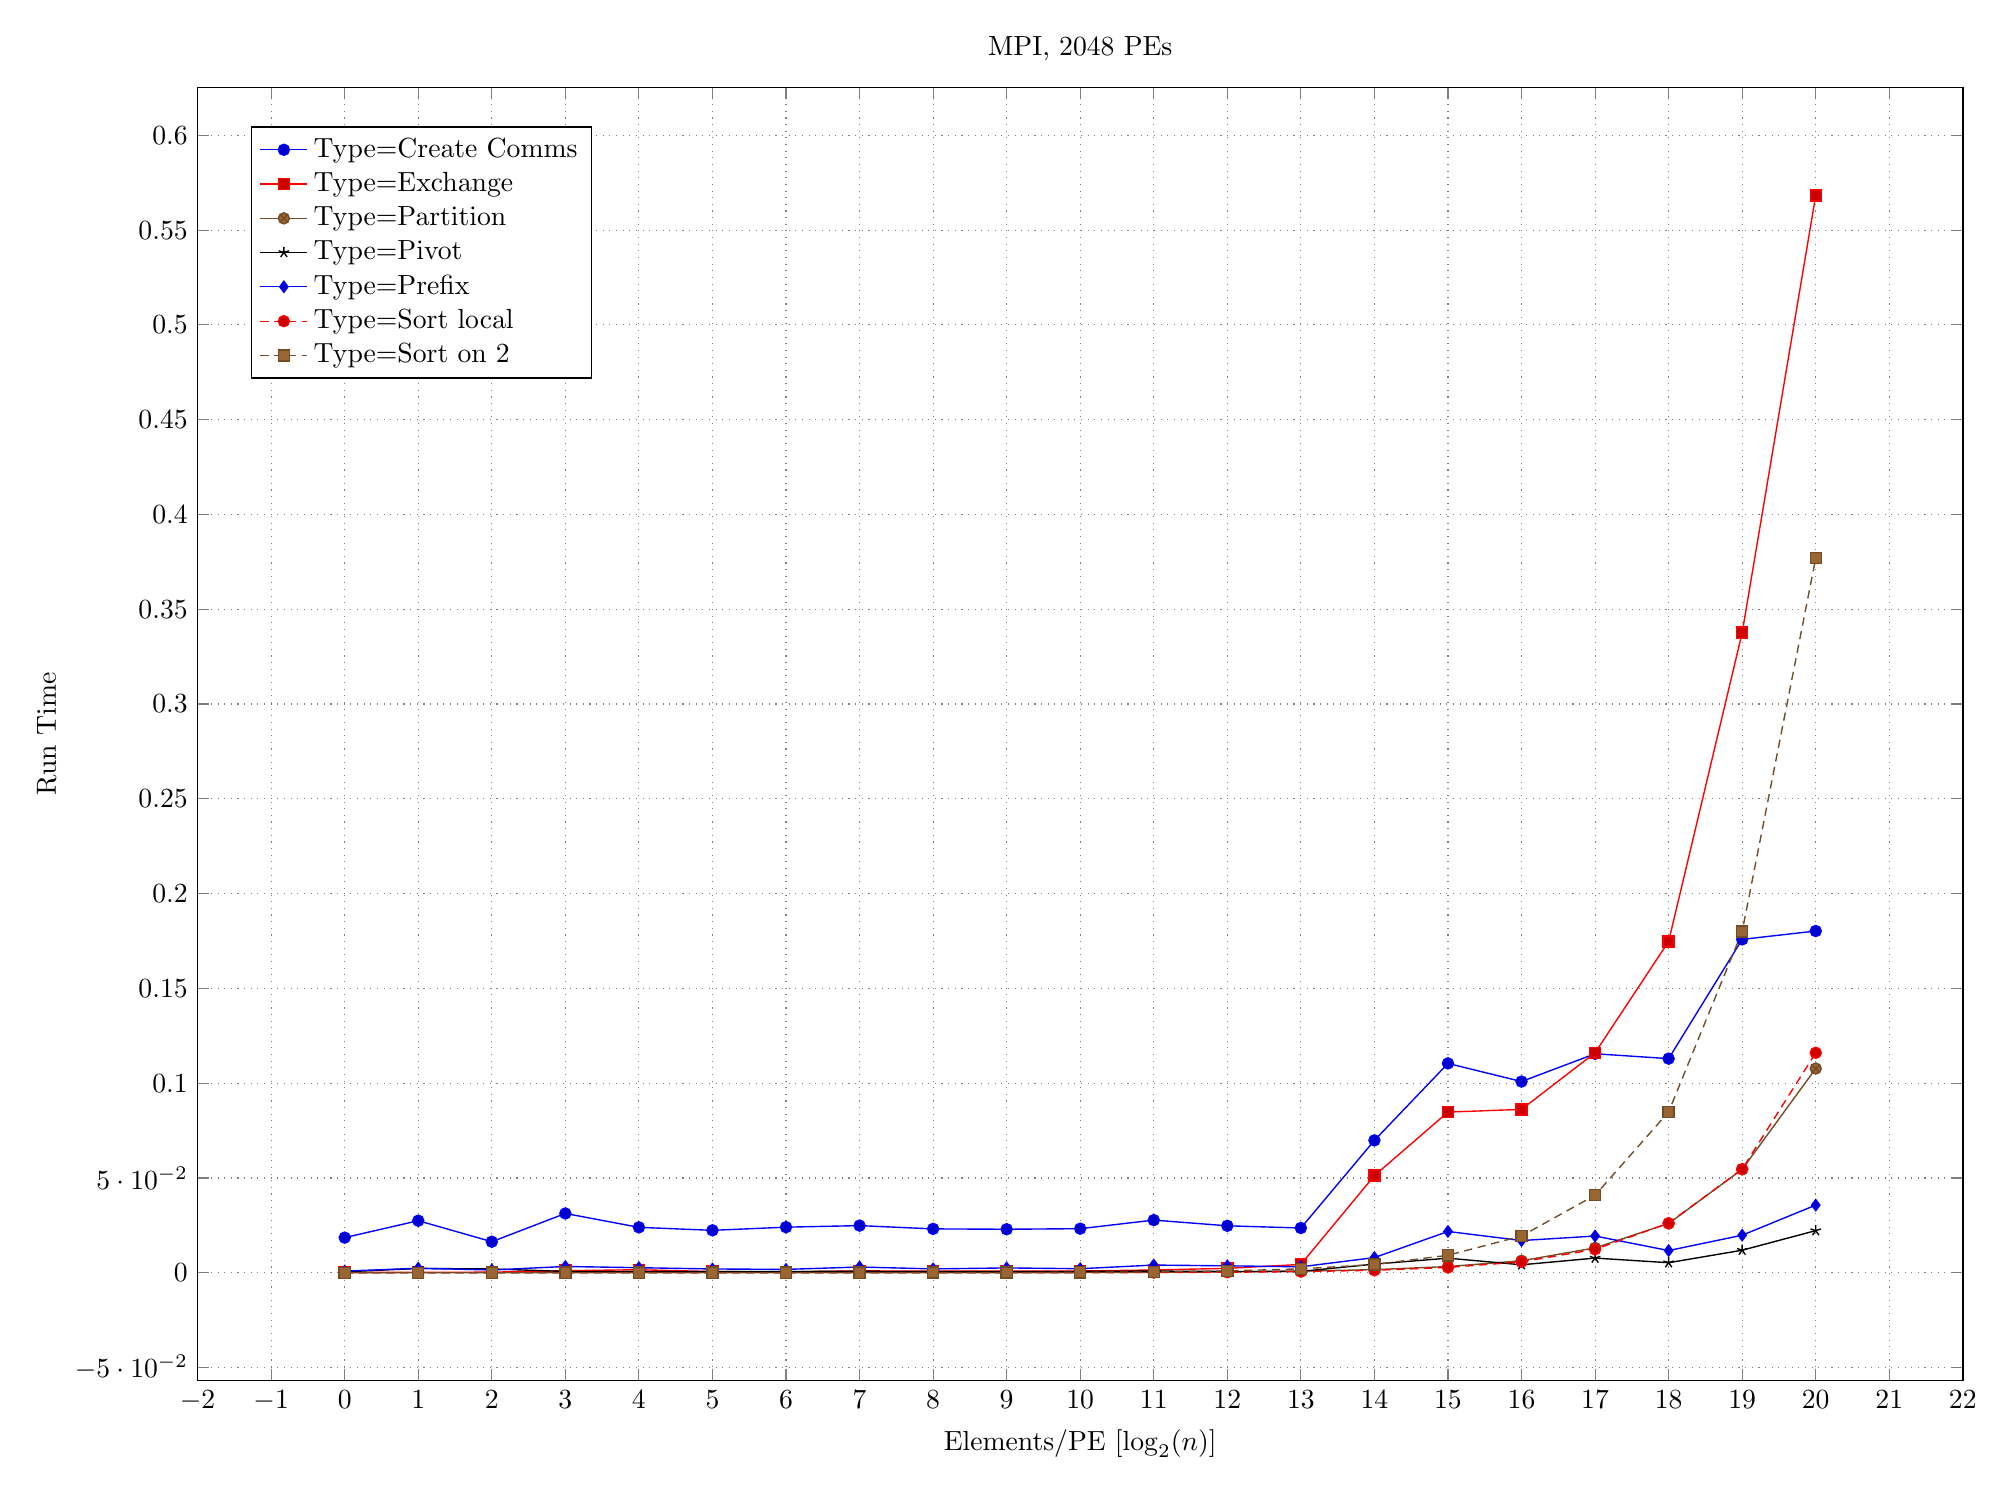
\begin{tikzpicture}
  \begin{axis}[
    title={MPI, 2048 PEs},
    xlabel={Elements/PE [$\log_2(n)$]},
    ylabel={Run Time},
    ]   
	%% MULTIPLOT(Type) SELECT size, collective, LOG(2,elements) AS x, Time as y, MULTIPLOT FROM (    
	%% SELECT elements, size, MEDIAN(pivot) as Time, 'Pivot' as Type, collective
	%% FROM ResultsQS
	%% GROUP BY collective, size, elements
	%% UNION ALL
	%% SELECT elements, size, MEDIAN(partition) as Time, 'Partition' as Type, collective
	%% FROM ResultsQS
	%% GROUP BY collective, size, elements
	%% UNION ALL
	%% SELECT elements, size, MEDIAN(calculate) as Time, 'Prefix' as Type, collective
	%% FROM ResultsQS
	%% GROUP BY collective, size, elements
	%% UNION ALL
	%% SELECT elements, size, MEDIAN(exchange) as Time, 'Exchange' as Type, collective
	%% FROM ResultsQS
	%% GROUP BY collective, size, elements
	%% UNION ALL
	%% SELECT elements, size, MEDIAN(create_comms) as Time, 'Create Comms' as Type, collective
	%% FROM ResultsQS
	%% GROUP BY collective, size, elements
	%% UNION ALL
	%% SELECT elements, size, MEDIAN(sort_two) as Time, 'Sort on 2' as Type, collective
	%% FROM ResultsQS
	%% GROUP BY collective, size, elements
	%% UNION ALL
	%% SELECT elements, size, MEDIAN(sort_local) as Time, 'Sort local' as Type, collective
	%% FROM ResultsQS
	%% GROUP BY collective, size, elements
	%% ) a
	%% WHERE collective="mpi" AND size=2048
	%% GROUP BY MULTIPLOT, x  ORDER BY MULTIPLOT, x
 \addplot coordinates { (0.0,0.0185403) (1.0,0.0274676) (2.0,0.0163795) (3.0,0.0312834) (4.0,0.023969) (5.0,0.022385) (6.0,0.0240554) (7.0,0.0248753) (8.0,0.0231484) (9.0,0.0229543) (10.0,0.0232588) (11.0,0.0277824) (12.0,0.0247744) (13.0,0.0236128) (14.0,0.0698361) (15.0,0.110434) (16.0,0.100875) (17.0,0.115524) (18.0,0.112954) (19.0,0.175868) (20.0,0.180269) };
 \addlegendentry{Type=Create Comms};
 \addplot coordinates { (0.0,0.000204237) (1.0,0.000257977) (2.0,0.000320004) (3.0,0.00109092) (4.0,0.00160318) (5.0,0.000637228) (6.0,0.000453684) (7.0,0.00101042) (8.0,0.000842773) (9.0,0.000870502) (10.0,0.00094209) (11.0,0.00146894) (12.0,0.00232615) (13.0,0.00440555) (14.0,0.0512415) (15.0,0.0847641) (16.0,0.0861871) (17.0,0.116047) (18.0,0.174777) (19.0,0.337655) (20.0,0.568296) };
 \addlegendentry{Type=Exchange};
 \addplot coordinates { (0.0,1.85519e-06) (1.0,4.94253e-06) (2.0,2.63005e-06) (3.0,8.93697e-06) (4.0,9.26666e-06) (5.0,1.48565e-05) (6.0,1.57114e-05) (7.0,2.51327e-05) (8.0,3.79076e-05) (9.0,5.91501e-05) (10.0,0.000112019) (11.0,0.000218759) (12.0,0.000425592) (13.0,0.000854445) (14.0,0.00164972) (15.0,0.00328962) (16.0,0.00633024) (17.0,0.0131386) (18.0,0.0260035) (19.0,0.0545563) (20.0,0.107729) };
 \addlegendentry{Type=Partition};
 \addplot coordinates { (0.0,0.000503142) (1.0,0.00226494) (2.0,0.00202023) (3.0,0.00069031) (4.0,0.000667724) (5.0,0.000642261) (6.0,0.000684614) (7.0,0.000728048) (8.0,0.000627981) (9.0,0.000623483) (10.0,0.000693594) (11.0,0.000884847) (12.0,0.000682798) (13.0,0.000723096) (14.0,0.0045649) (15.0,0.00770314) (16.0,0.00420924) (17.0,0.0077424) (18.0,0.00530064) (19.0,0.0118974) (20.0,0.0222273) };
 \addlegendentry{Type=Pivot};
 \addplot coordinates { (0.0,0.00087704) (1.0,0.00239512) (2.0,0.00146734) (3.0,0.0033241) (4.0,0.002675) (5.0,0.00200183) (6.0,0.00177798) (7.0,0.00304266) (8.0,0.00204044) (9.0,0.00255191) (10.0,0.00214582) (11.0,0.00406442) (12.0,0.00365871) (13.0,0.00314152) (14.0,0.00800985) (15.0,0.0217868) (16.0,0.0169977) (17.0,0.019388) (18.0,0.0117154) (19.0,0.0198114) (20.0,0.0356952) };
 \addlegendentry{Type=Prefix};
 \addplot coordinates { (0.0,3.1665e-07) (1.0,4.46103e-07) (2.0,4.67524e-07) (3.0,5.68106e-07) (4.0,7.3947e-07) (5.0,1.47522e-06) (6.0,2.82377e-06) (7.0,6.12624e-06) (8.0,1.32974e-05) (9.0,2.8939e-05) (10.0,5.97956e-05) (11.0,0.000133343) (12.0,0.000285615) (13.0,0.000613659) (14.0,0.00131462) (15.0,0.00281371) (16.0,0.00577427) (17.0,0.0123582) (18.0,0.0261472) (19.0,0.0546452) (20.0,0.116034) };
 \addlegendentry{Type=Sort local};
 \addplot coordinates { (0.0,1.90121e-05) (1.0,2.13692e-05) (2.0,2.75942e-05) (3.0,2.45329e-05) (4.0,2.69674e-05) (5.0,2.98638e-05) (6.0,3.43723e-05) (7.0,4.46951e-05) (8.0,6.61165e-05) (9.0,0.000114893) (10.0,0.000228697) (11.0,0.000468338) (12.0,0.000968074) (13.0,0.00207009) (14.0,0.00435857) (15.0,0.00921726) (16.0,0.0193775) (17.0,0.0408977) (18.0,0.084849) (19.0,0.180026) (20.0,0.376924) };
 \addlegendentry{Type=Sort on 2};

  \end{axis}
\end{tikzpicture}
\newpage

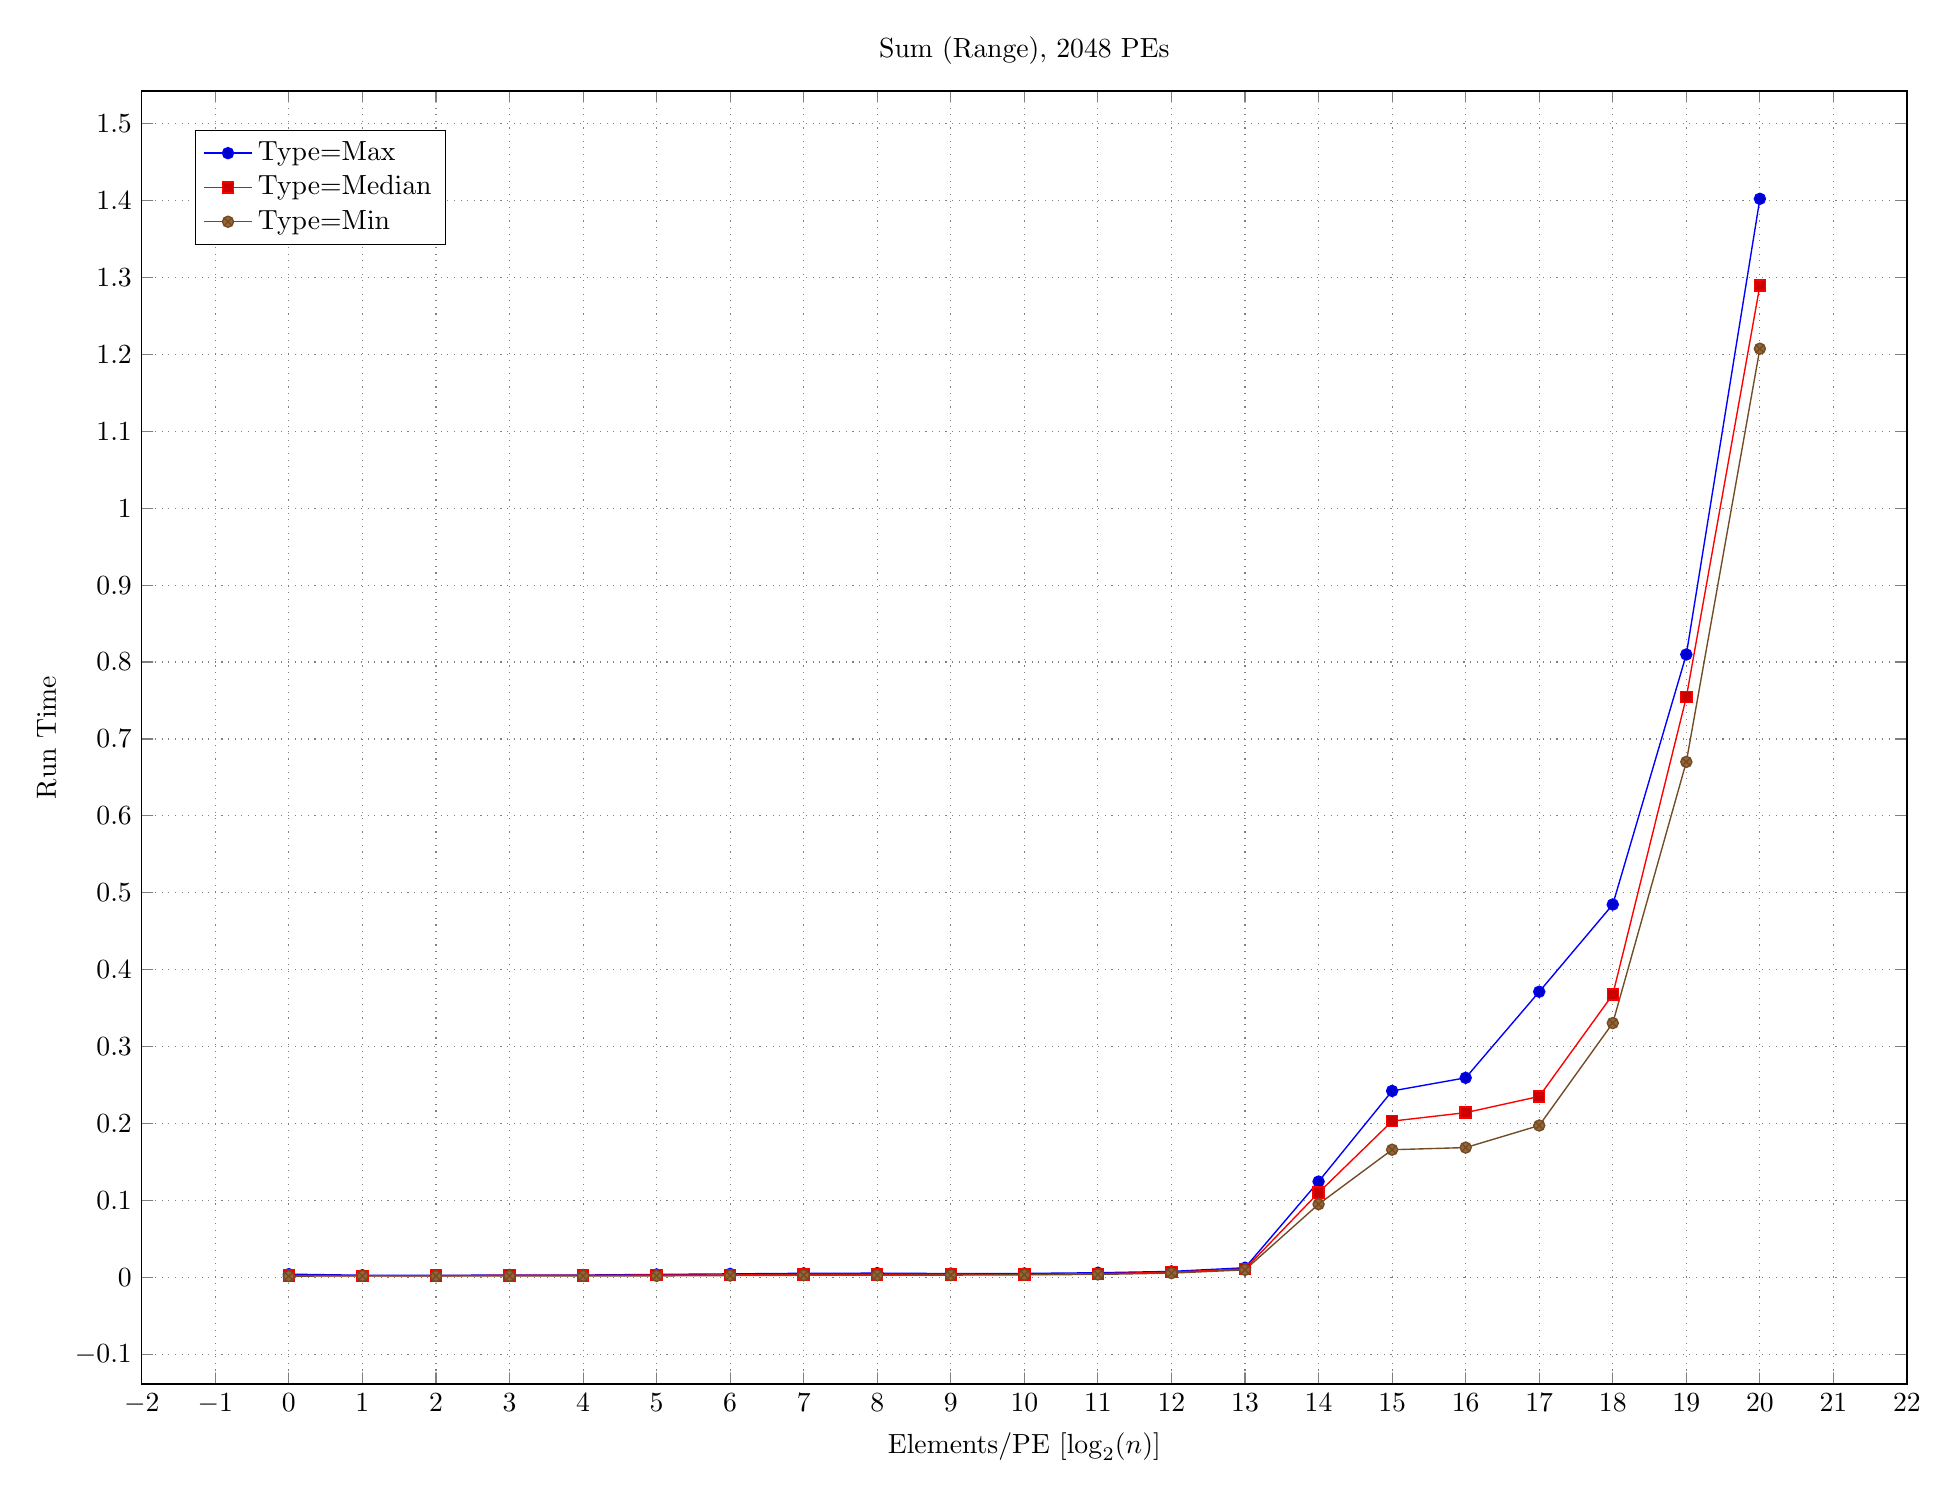
\begin{tikzpicture}
  \begin{axis}[
    title={Sum (Range), 2048 PEs},
    xlabel={Elements/PE [$\log_2(n)$]},
    ylabel={Run Time},
    ]   
	%% MULTIPLOT(Type) SELECT size, collective, LOG(2,elements) AS x, Time as y, MULTIPLOT FROM (    
	%% SELECT elements, size, MEDIAN(sum) as Time, 'Median' as Type, collective
	%% FROM ResultsQS
	%% GROUP BY collective, size, elements
	%% UNION ALL
	%% SELECT elements, size, MIN(sum) as Time, 'Min' as Type, collective
	%% FROM ResultsQS
	%% GROUP BY collective, size, elements
	%% UNION ALL    
	%% SELECT elements, size, MAX(sum) as Time, 'Max' as Type, collective
	%% FROM ResultsQS
	%% GROUP BY collective, size, elements
	%% ) a
	%% WHERE collective="range" AND size=2048
	%% GROUP BY MULTIPLOT, x  ORDER BY MULTIPLOT, x
 \addplot coordinates { (0.0,0.0041381) (1.0,0.0027279) (2.0,0.0025349) (3.0,0.0031001) (4.0,0.00300047) (5.0,0.00379676) (6.0,0.00450842) (7.0,0.00523819) (8.0,0.00545529) (9.0,0.004897) (10.0,0.00507859) (11.0,0.00598805) (12.0,0.00770284) (13.0,0.0124702) (14.0,0.12454) (15.0,0.242336) (16.0,0.259433) (17.0,0.371365) (18.0,0.484772) (19.0,0.809838) (20.0,1.40227) };
 \addlegendentry{Type=Max};
 \addplot coordinates { (0.0,0.00248972) (1.0,0.00207575) (2.0,0.0021612) (3.0,0.00263017) (4.0,0.00250626) (5.0,0.00296712) (6.0,0.00303747) (7.0,0.00382616) (8.0,0.00384842) (9.0,0.00385053) (10.0,0.003638) (11.0,0.00462792) (12.0,0.0066758) (13.0,0.0108683) (14.0,0.110065) (15.0,0.203104) (16.0,0.214144) (17.0,0.235226) (18.0,0.367683) (19.0,0.754289) (20.0,1.289525) };
 \addlegendentry{Type=Median};
 \addplot coordinates { (0.0,0.00157808) (1.0,0.00187625) (2.0,0.00175364) (3.0,0.00187074) (4.0,0.00182845) (5.0,0.00190682) (6.0,0.00230771) (7.0,0.00271828) (8.0,0.00272179) (9.0,0.00292046) (10.0,0.00328367) (11.0,0.00381874) (12.0,0.00548646) (13.0,0.0097251) (14.0,0.0951028) (15.0,0.165939) (16.0,0.168724) (17.0,0.197415) (18.0,0.330607) (19.0,0.670207) (20.0,1.20741) };
 \addlegendentry{Type=Min};

  \end{axis}
\end{tikzpicture}
\newpage

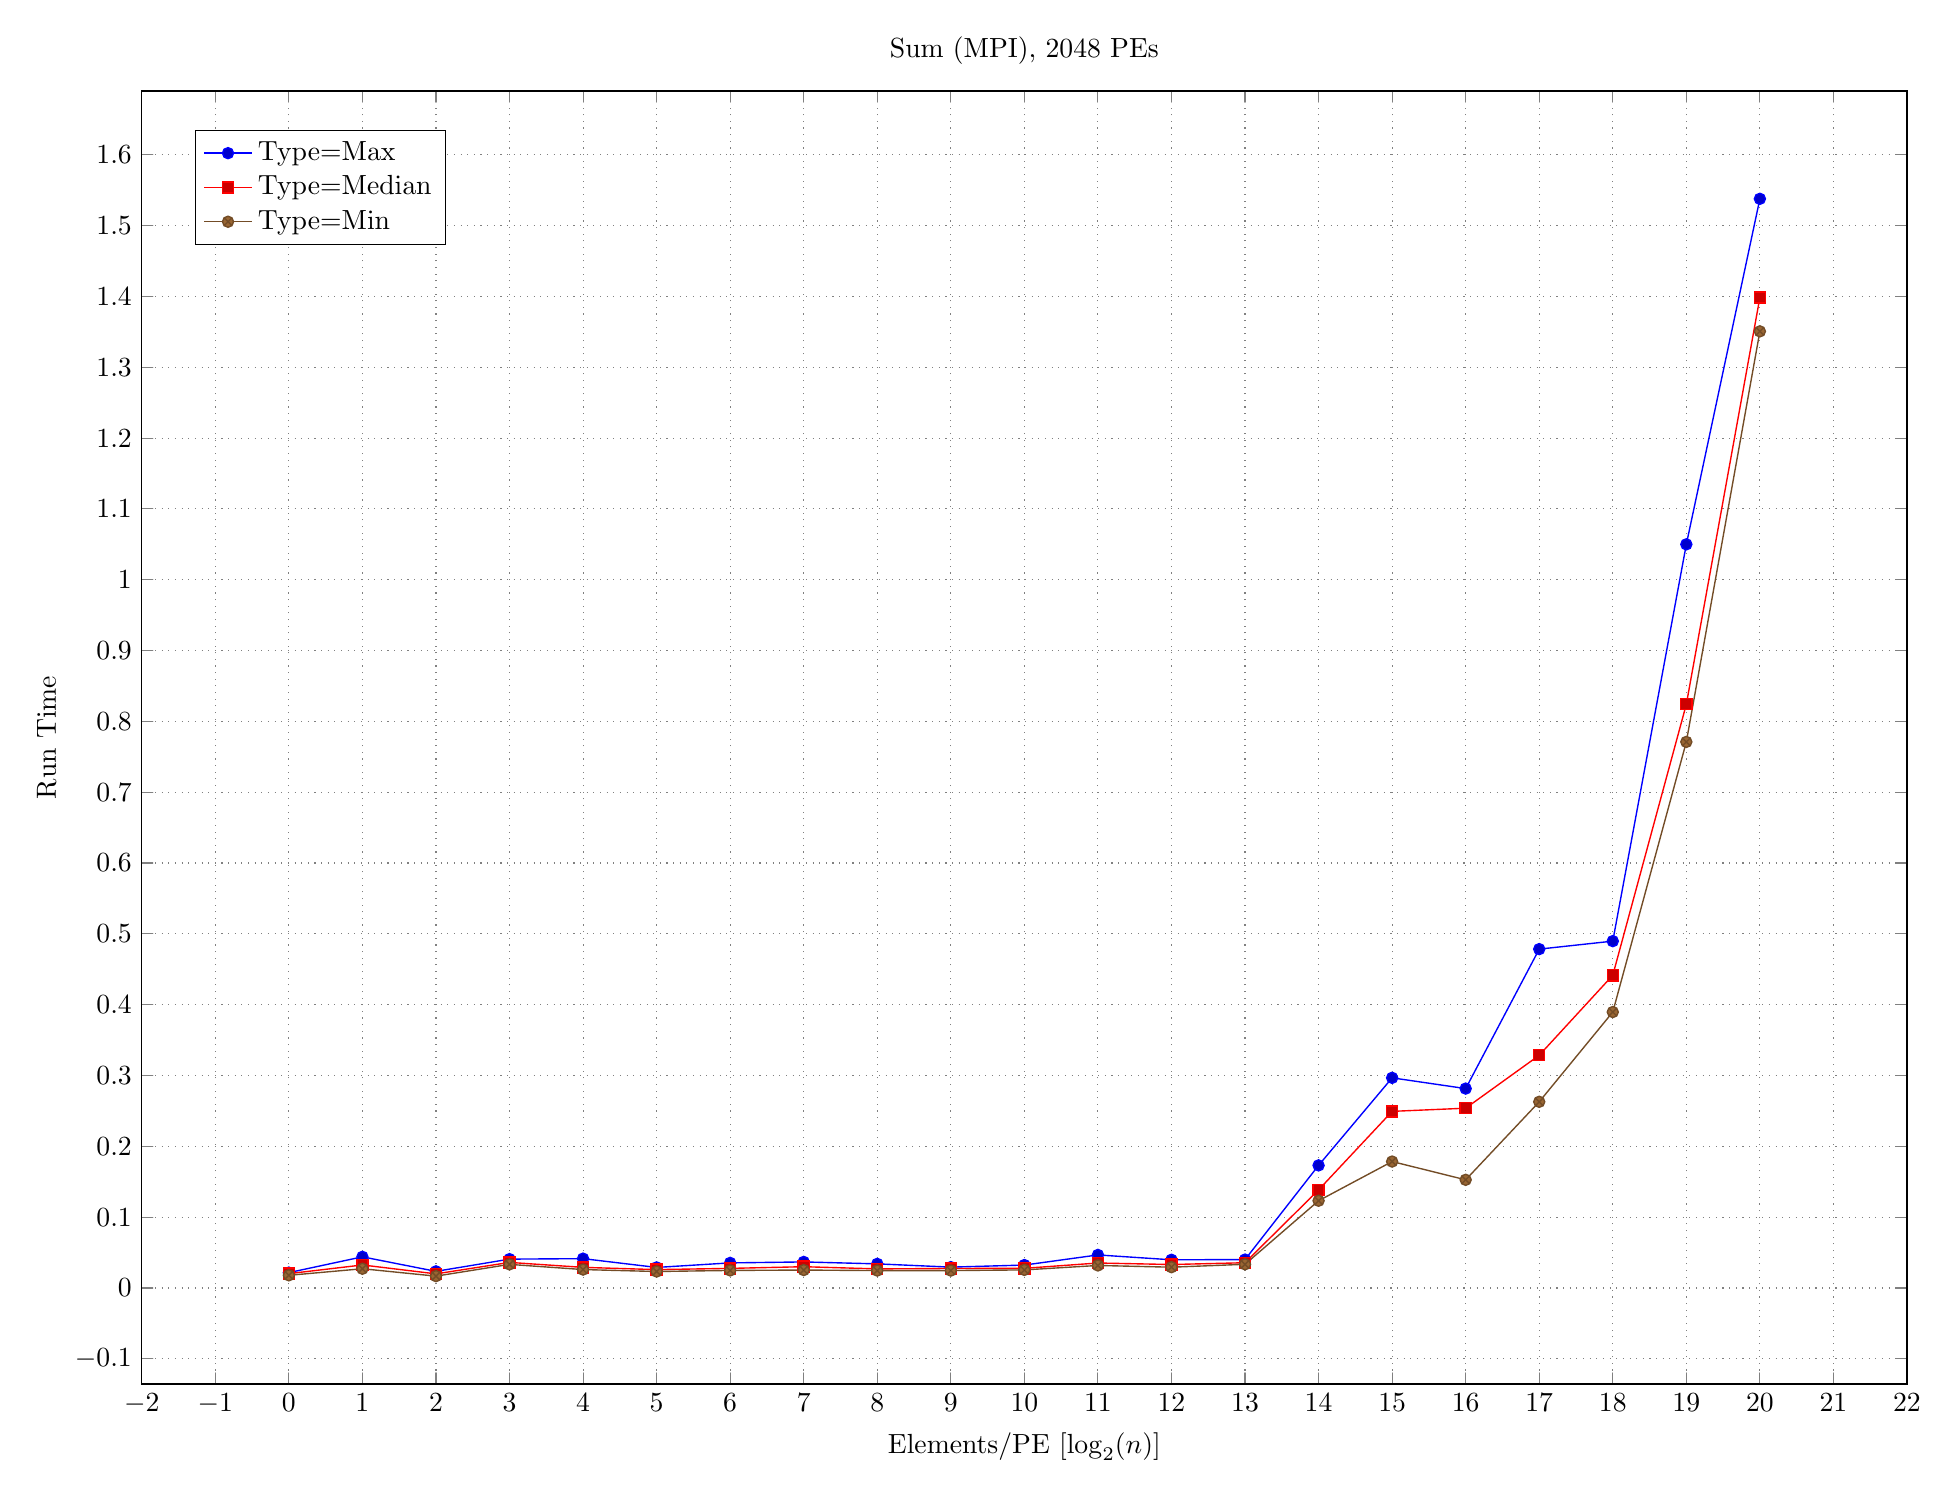
\begin{tikzpicture}
  \begin{axis}[
    title={Sum (MPI), 2048 PEs},
    xlabel={Elements/PE [$\log_2(n)$]},
    ylabel={Run Time},
    ]   
	%% MULTIPLOT(Type) SELECT size, collective, LOG(2,elements) AS x, Time as y, MULTIPLOT FROM (    
	%% SELECT elements, size, MEDIAN(sum) as Time, 'Median' as Type, collective
	%% FROM ResultsQS
	%% GROUP BY collective, size, elements
	%% UNION ALL
	%% SELECT elements, size, MIN(sum) as Time, 'Min' as Type, collective
	%% FROM ResultsQS
	%% GROUP BY collective, size, elements
	%% UNION ALL    
	%% SELECT elements, size, MAX(sum) as Time, 'Max' as Type, collective
	%% FROM ResultsQS
	%% GROUP BY collective, size, elements
	%% ) a
	%% WHERE collective="mpi" AND size=2048
	%% GROUP BY MULTIPLOT, x  ORDER BY MULTIPLOT, x
 \addplot coordinates { (0.0,0.0216414) (1.0,0.0439514) (2.0,0.0234229) (3.0,0.0406997) (4.0,0.0413837) (5.0,0.0289794) (6.0,0.0353873) (7.0,0.036743) (8.0,0.0340152) (9.0,0.0294058) (10.0,0.0323205) (11.0,0.0466232) (12.0,0.0397765) (13.0,0.040071) (14.0,0.173066) (15.0,0.296693) (16.0,0.281499) (17.0,0.478441) (18.0,0.489713) (19.0,1.05) (20.0,1.53788) };
 \addlegendentry{Type=Max};
 \addplot coordinates { (0.0,0.0201961) (1.0,0.0324485) (2.0,0.0198806) (3.0,0.036062) (4.0,0.0290707) (5.0,0.0259023) (6.0,0.027636) (7.0,0.0300001) (8.0,0.0269185) (9.0,0.0274694) (10.0,0.0277356) (11.0,0.035226) (12.0,0.0330935) (13.0,0.0356159) (14.0,0.138453) (15.0,0.249352) (16.0,0.253815) (17.0,0.328552) (18.0,0.441508) (19.0,0.824168) (20.0,1.39854) };
 \addlegendentry{Type=Median};
 \addplot coordinates { (0.0,0.0178414) (1.0,0.0271104) (2.0,0.016682) (3.0,0.0332797) (4.0,0.0259707) (5.0,0.0232129) (6.0,0.0247398) (7.0,0.0252665) (8.0,0.024555) (9.0,0.0245357) (10.0,0.0254945) (11.0,0.0317567) (12.0,0.0293177) (13.0,0.0334024) (14.0,0.123145) (15.0,0.178499) (16.0,0.152699) (17.0,0.262866) (18.0,0.389603) (19.0,0.771035) (20.0,1.35074) };
 \addlegendentry{Type=Min};

  \end{axis}
\end{tikzpicture}
\newpage

\begin{tikzpicture}
  \begin{axis}[
    title={Median of Sum, 2048 PEs},
    xlabel={Elements / PE [$\log_2(n)$]},
    ylabel={Run Time},
    ]   
	%% MULTIPLOT(collective) SELECT collective, LOG(2,elements) AS x, MEDIAN(sum) as y
	%% FROM ResultsQS
	%% WHERE size=2048 
	%% GROUP BY MULTIPLOT, x  ORDER BY MULTIPLOT, x
 \addplot coordinates { (0.0,0.0201961) (1.0,0.0324485) (2.0,0.0198806) (3.0,0.036062) (4.0,0.0290707) (5.0,0.0259023) (6.0,0.027636) (7.0,0.0300001) (8.0,0.0269185) (9.0,0.0274694) (10.0,0.0277356) (11.0,0.035226) (12.0,0.0330935) (13.0,0.0356159) (14.0,0.138453) (15.0,0.249352) (16.0,0.253815) (17.0,0.328552) (18.0,0.441508) (19.0,0.824168) (20.0,1.39854) };
 \addlegendentry{collective=mpi};
 \addplot coordinates { (0.0,0.00248972) (1.0,0.00207575) (2.0,0.0021612) (3.0,0.00263017) (4.0,0.00250626) (5.0,0.00296712) (6.0,0.00303747) (7.0,0.00382616) (8.0,0.00384842) (9.0,0.00385053) (10.0,0.003638) (11.0,0.00462792) (12.0,0.0066758) (13.0,0.0108683) (14.0,0.110065) (15.0,0.203104) (16.0,0.214144) (17.0,0.235226) (18.0,0.367683) (19.0,0.754289) (20.0,1.289525) };
 \addlegendentry{collective=range};

  \end{axis}
\end{tikzpicture}

\begin{tikzpicture}
\begin{axis}[
title={Median of Sum, $2^{25}$ total elements},
xlabel={PEs [$\log_2(n)$]},
ylabel={Run Time},
]   
%% MULTIPLOT(collective) SELECT elements*size AS total_elements, collective, LOG(2,size) AS x, MEDIAN(sum) as y
%% FROM ResultsQS
%% WHERE total_elements=POWER(2,25)
%% GROUP BY MULTIPLOT, x  ORDER BY MULTIPLOT, x
\addplot coordinates { (6.0,0.322044) (7.0,0.183614) (8.0,0.113569) (9.0,0.0905592) (10.0,0.147741) (11.0,0.138453) (13.0,0.413542) };
\addlegendentry{collective=mpi};
\addplot coordinates { (6.0,0.320823) (7.0,0.175193) (8.0,0.107829) (9.0,0.112197) (10.0,0.136777) (11.0,0.110065) (13.0,0.0103032) };
\addlegendentry{collective=range};

\end{axis}
\end{tikzpicture}

\begin{tikzpicture}
  \begin{axis}[
    title={Pivot (Range)},
    xlabel={PEs [$\log_2(n)$]},
    ylabel={Run Time},
    ]   
	%% MULTIPLOT(Type) SELECT elements, collective, LOG(2,size) AS x, Time as y, MULTIPLOT FROM (    
	%% SELECT elements, size, MEDIAN(pivot) as Time, 'Median' as Type, collective
	%% FROM ResultsQS
	%% GROUP BY collective, size, elements
	%% UNION ALL
	%% SELECT elements, size, MIN(pivot) as Time, 'Min' as Type, collective
	%% FROM ResultsQS
	%% GROUP BY collective, size, elements
	%% UNION ALL    
	%% SELECT elements, size, MAX(pivot) as Time, 'Max' as Type, collective
	%% FROM ResultsQS
	%% GROUP BY collective, size, elements
	%% ) a
	%% WHERE collective="range"
	%% GROUP BY MULTIPLOT, x  ORDER BY MULTIPLOT, x
 \addplot coordinates { (6.0,0.0061012) (7.0,0.0309154) (8.0,0.0690706) (9.0,0.0964464) (10.0,0.151537) (11.0,0.131031) (13.0,0.284004) };
 \addlegendentry{Type=Max};
 \addplot coordinates { (6.0,0.0040016) (7.0,0.0193228) (8.0,0.0241468) (9.0,0.052234) (10.0,0.0778279) (11.0,0.0775652) (13.0,0.13096) };
 \addlegendentry{Type=Median};
 \addplot coordinates { (6.0,0.00164558) (7.0,0.00935364) (8.0,0.00854798) (9.0,0.0321084) (10.0,0.0480165) (11.0,0.0430164) (13.0,0.0610251) };
 \addlegendentry{Type=Min};

  \end{axis}
\end{tikzpicture}
\newpage

\begin{tikzpicture}
  \begin{axis}[
    title={Pivot (MPI)},
    xlabel={PEs [$\log_2(n)$]},
    ylabel={Run Time},
    ]   
	%% MULTIPLOT(Type) SELECT elements, collective, LOG(2,size) AS x, Time as y, MULTIPLOT FROM (    
	%% SELECT elements, size, MEDIAN(pivot) as Time, 'Median' as Type, collective
	%% FROM ResultsQS
	%% GROUP BY collective, size, elements
	%% UNION ALL
	%% SELECT elements, size, MIN(pivot) as Time, 'Min' as Type, collective
	%% FROM ResultsQS
	%% GROUP BY collective, size, elements
	%% UNION ALL    
	%% SELECT elements, size, MAX(pivot) as Time, 'Max' as Type, collective
	%% FROM ResultsQS
	%% GROUP BY collective, size, elements
	%% ) a
	%% WHERE collective="mpi"
	%% GROUP BY MULTIPLOT, x  ORDER BY MULTIPLOT, x
 \addplot coordinates { (6.0,0.00180984) (7.0,0.0172524) (8.0,0.0298247) (9.0,0.0267193) (10.0,0.0251434) (11.0,0.0280635) (13.0,0.0757958) };
 \addlegendentry{Type=Max};
 \addplot coordinates { (6.0,0.000367634) (7.0,0.0041966) (8.0,0.0137521) (9.0,0.0114884) (10.0,0.013606) (11.0,0.0222273) (13.0,0.0331757) };
 \addlegendentry{Type=Median};
 \addplot coordinates { (6.0,0.000294412) (7.0,0.000370722) (8.0,0.000759536) (9.0,0.00110203) (10.0,0.011716) (11.0,0.00785135) (13.0,0.0246996) };
 \addlegendentry{Type=Min};

  \end{axis}
\end{tikzpicture}
\newpage

\begin{tikzpicture}
  \begin{axis}[
    title={Prefix sum (Range)},
    xlabel={PEs [$\log_2(n)$]},
    ylabel={Run Time},
    ]   
	%% MULTIPLOT(Type) SELECT elements, collective, LOG(2,size) AS x, Time as y, MULTIPLOT FROM (    
	%% SELECT elements, size, MEDIAN(calculate) as Time, 'Median' as Type, collective
	%% FROM ResultsQS
	%% GROUP BY collective, size, elements
	%% UNION ALL
	%% SELECT elements, size, MIN(calculate) as Time, 'Min' as Type, collective
	%% FROM ResultsQS
	%% GROUP BY collective, size, elements
	%% UNION ALL    
	%% SELECT elements, size, MAX(calculate) as Time, 'Max' as Type, collective
	%% FROM ResultsQS
	%% GROUP BY collective, size, elements
	%% ) a
	%% WHERE collective="range"
	%% GROUP BY MULTIPLOT, x  ORDER BY MULTIPLOT, x
 \addplot coordinates { (6.0,0.0119515) (7.0,0.0331175) (8.0,0.0306056) (9.0,0.0315476) (10.0,0.0952374) (11.0,0.0638708) (13.0,0.125413) };
 \addlegendentry{Type=Max};
 \addplot coordinates { (6.0,0.00864934) (7.0,0.0237042) (8.0,0.0193636) (9.0,0.0211961) (10.0,0.0385763) (11.0,0.0411422) (13.0,0.0923424) };
 \addlegendentry{Type=Median};
 \addplot coordinates { (6.0,0.00548968) (7.0,0.00735969) (8.0,0.014371) (9.0,0.0172015) (10.0,0.0294958) (11.0,0.0308945) (13.0,0.072068) };
 \addlegendentry{Type=Min};

  \end{axis}
\end{tikzpicture}
\newpage

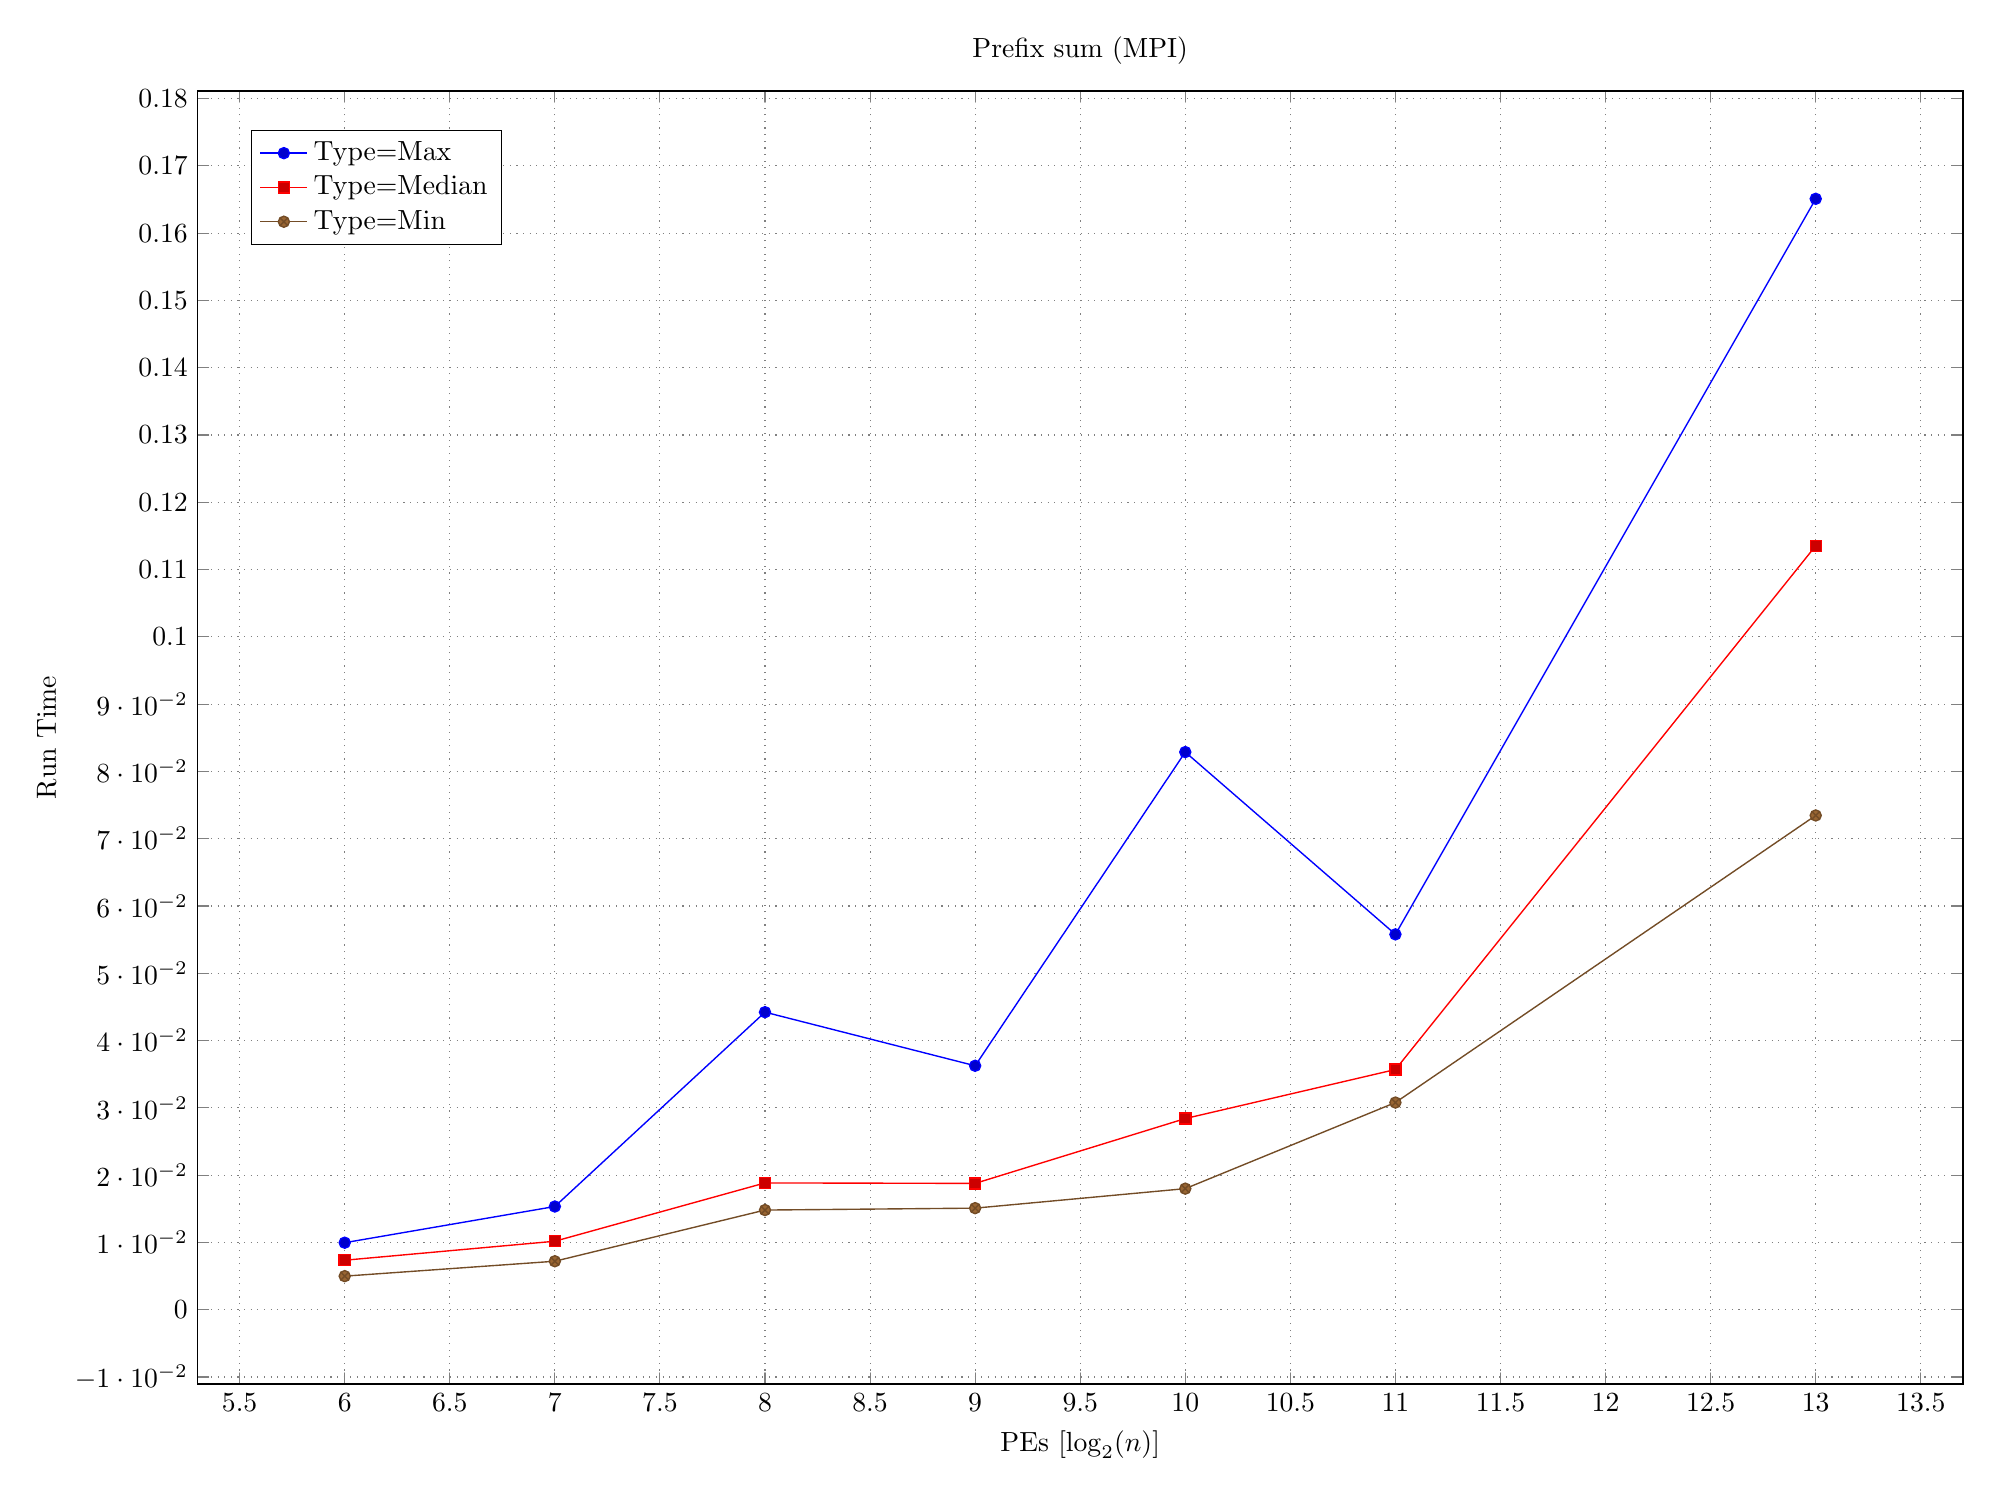
\begin{tikzpicture}
  \begin{axis}[
    title={Prefix sum (MPI)},
    xlabel={PEs [$\log_2(n)$]},
    ylabel={Run Time},
    ]   
	%% MULTIPLOT(Type) SELECT elements, collective, LOG(2,size) AS x, Time as y, MULTIPLOT FROM (    
	%% SELECT elements, size, MEDIAN(calculate) as Time, 'Median' as Type, collective
	%% FROM ResultsQS
	%% GROUP BY collective, size, elements
	%% UNION ALL
	%% SELECT elements, size, MIN(calculate) as Time, 'Min' as Type, collective
	%% FROM ResultsQS
	%% GROUP BY collective, size, elements
	%% UNION ALL    
	%% SELECT elements, size, MAX(calculate) as Time, 'Max' as Type, collective
	%% FROM ResultsQS
	%% GROUP BY collective, size, elements
	%% ) a
	%% WHERE collective="mpi"
	%% GROUP BY MULTIPLOT, x  ORDER BY MULTIPLOT, x
 \addplot coordinates { (6.0,0.0099567) (7.0,0.0153367) (8.0,0.04422) (9.0,0.0362524) (10.0,0.0828759) (11.0,0.0557839) (13.0,0.165102) };
 \addlegendentry{Type=Max};
 \addplot coordinates { (6.0,0.00735342) (7.0,0.010175) (8.0,0.0188407) (9.0,0.0187714) (10.0,0.028407) (11.0,0.0356952) (13.0,0.113538) };
 \addlegendentry{Type=Median};
 \addplot coordinates { (6.0,0.00498737) (7.0,0.007202) (8.0,0.0148093) (9.0,0.0150926) (10.0,0.0179903) (11.0,0.0307875) (13.0,0.0734564) };
 \addlegendentry{Type=Min};

  \end{axis}
\end{tikzpicture}
\newpage

\begin{tikzpicture}
  \begin{axis}[
    title={Median of partition, $2^{25}$ total elements},
    xlabel={PEs [$\log_2(n)$]},
    ylabel={Run Time [$\log_2(n)$]},
    ]   
	%% MULTIPLOT(collective) SELECT collective, elements*size AS total_elements, LOG(2,size) AS x, MEDIAN(partition) as y
	%% FROM ResultsQS
	%% WHERE total_elements=POWER(2,25)
	%% GROUP BY MULTIPLOT, x ORDER BY MULTIPLOT, x
 \addplot coordinates { (6.0,0.0267397) (7.0,0.0160951) (8.0,0.00918919) (9.0,0.00522509) (10.0,0.00291289) (11.0,0.00164972) (13.0,0.000510117) };
 \addlegendentry{collective=mpi};
 \addplot coordinates { (6.0,0.0268227) (7.0,0.0160371) (8.0,0.00910693) (9.0,0.00507652) (10.0,0.00278854) (11.0,0.00161797) (13.0,0.000489571) };
 \addlegendentry{collective=range};
  \end{axis}
\end{tikzpicture}
\newpage

\begin{tikzpicture}
  \begin{axis}[
    title={Median of sort\_two, $2^{25}$ total elements},
    xlabel={PEs [$\log_2(n)$]},
    ylabel={Run Time [$\log_2(n)$]},
    ]   
	%% MULTIPLOT(collective) SELECT collective, elements*size AS total_elements, LOG(2,size) AS x, MEDIAN(sort_two) as y
	%% FROM ResultsQS
	%% WHERE total_elements=POWER(2,25)
	%% GROUP BY MULTIPLOT, x ORDER BY MULTIPLOT, x
 \addplot coordinates { (6.0,0.169611) (7.0,0.0816812) (8.0,0.0396859) (9.0,0.0189363) (10.0,0.0091597) (11.0,0.00435857) (13.0,0.000987884) };
 \addlegendentry{collective=mpi};
 \addplot coordinates { (6.0,0.171191) (7.0,0.0828334) (8.0,0.040639) (9.0,0.0191642) (10.0,0.00922053) (11.0,0.00438891) (13.0,0.000995412) };
 \addlegendentry{collective=range};
  \end{axis}
\end{tikzpicture}
\newpage

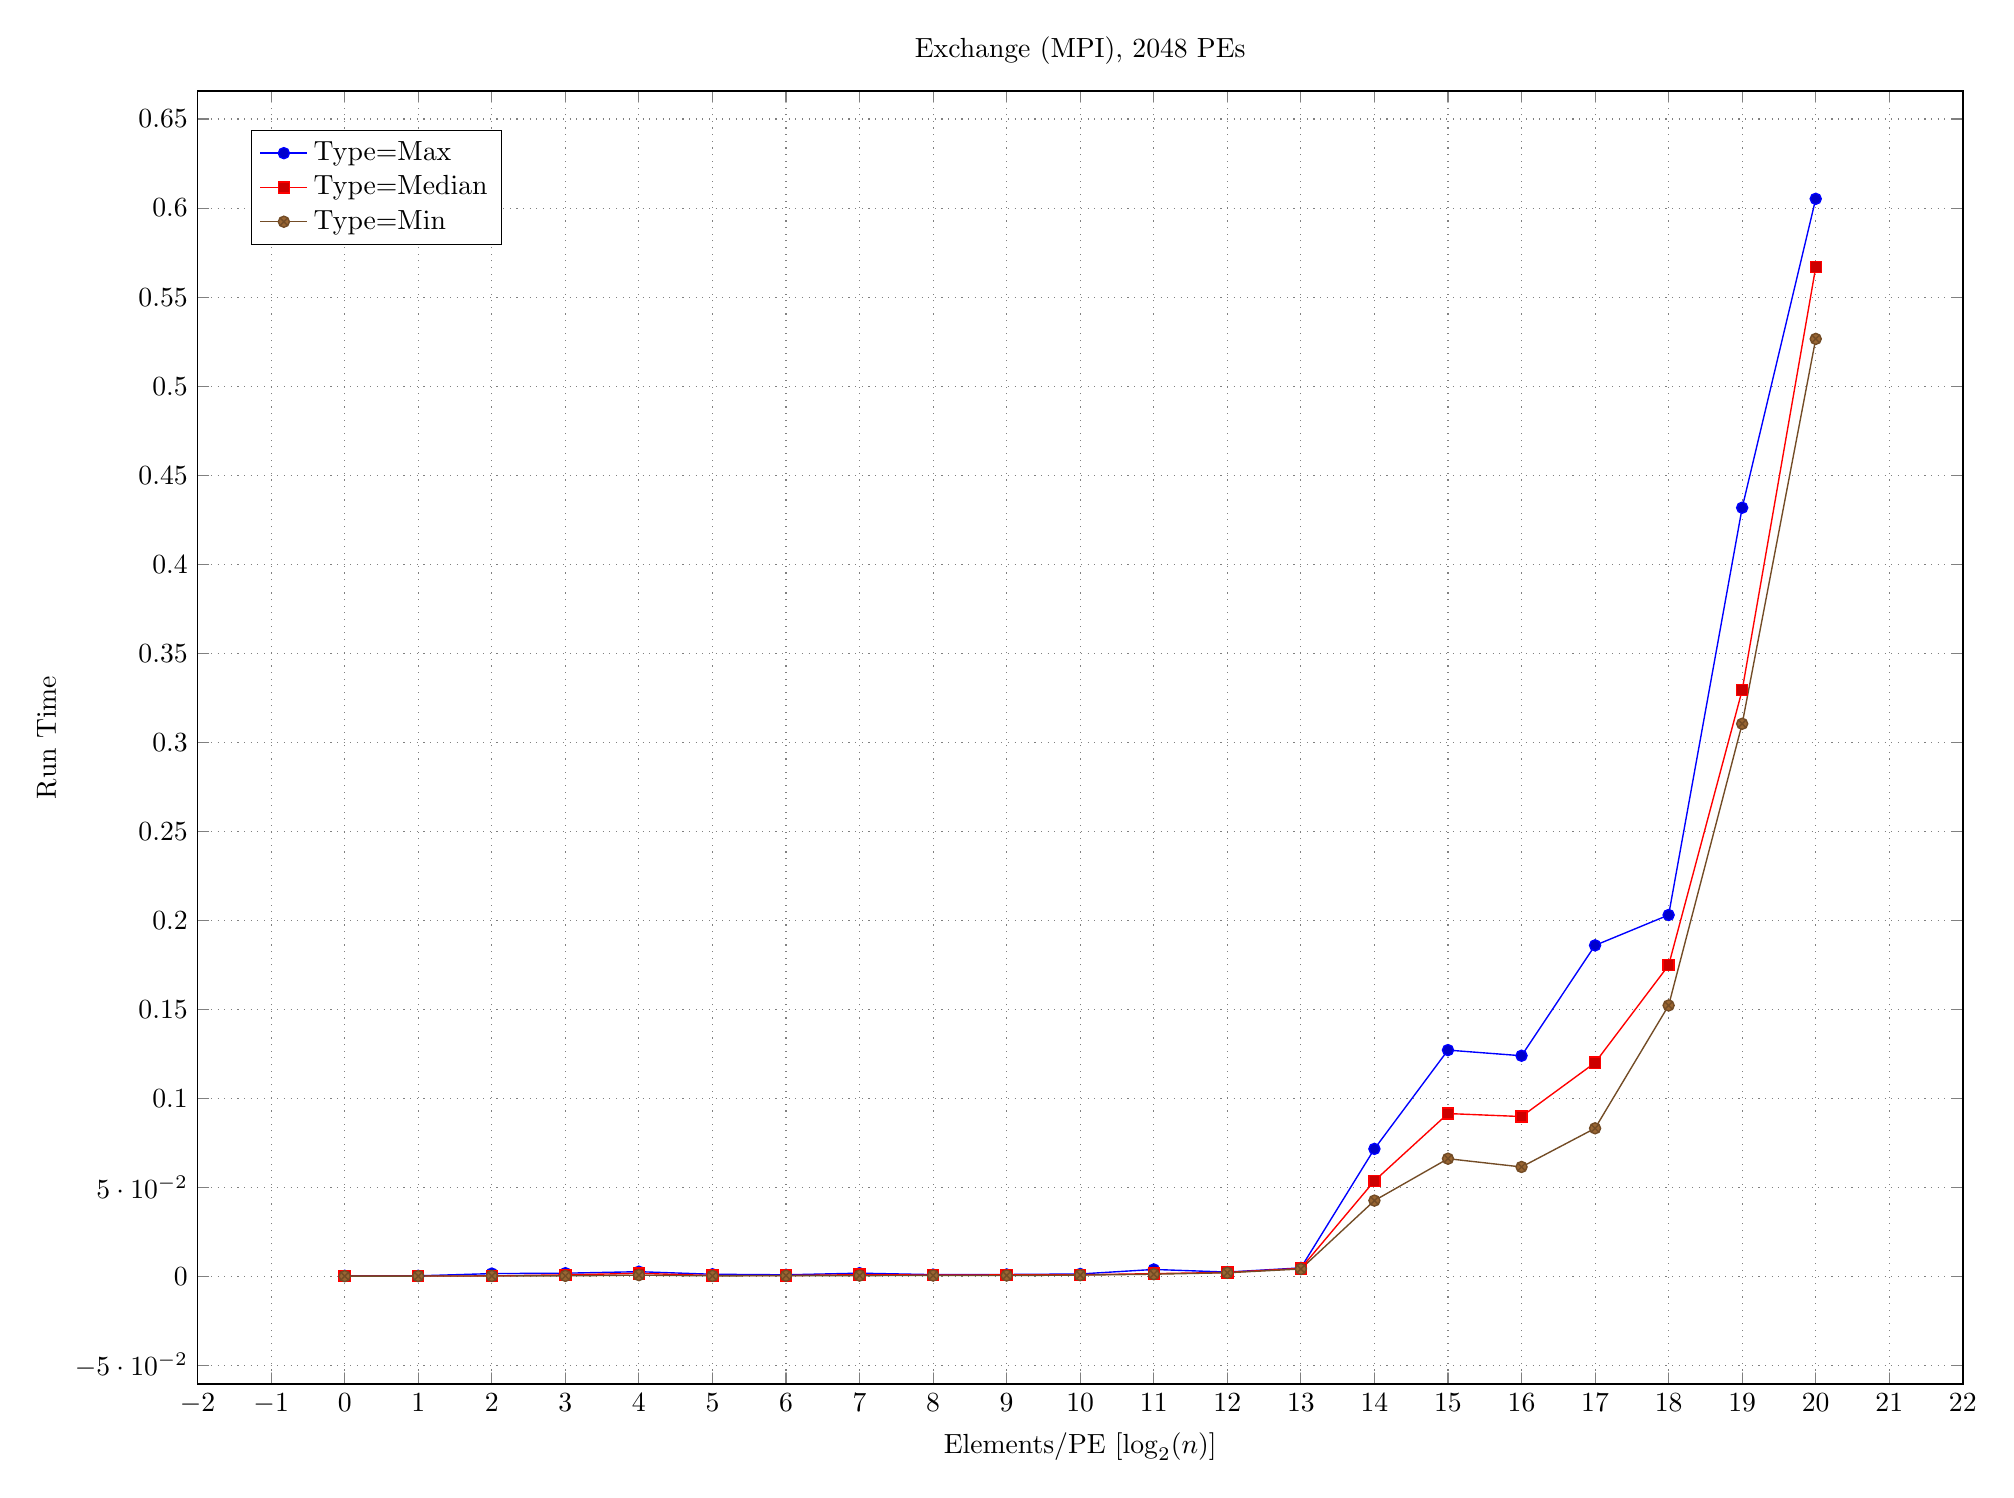
\begin{tikzpicture}
  \begin{axis}[
    title={Exchange (MPI), 2048 PEs},
    xlabel={Elements/PE [$\log_2(n)$]},
    ylabel={Run Time},
    ]   
	%% MULTIPLOT(Type) SELECT collective, size, LOG(2,elements) AS x, Time as y, MULTIPLOT FROM (    
	%% SELECT elements, size, MEDIAN(exchange) as Time, 'Median' as Type, collective
	%% FROM ResultsQS WHERE iteration>0
	%% GROUP BY collective, size, elements
	%% UNION ALL
	%% SELECT elements, size, MIN(exchange) as Time, 'Min' as Type, collective
	%% FROM ResultsQS WHERE iteration>0
	%% GROUP BY collective, size, elements
	%% UNION ALL    
	%% SELECT elements, size, MAX(exchange) as Time, 'Max' as Type, collective
	%% FROM ResultsQS WHERE iteration>0
	%% GROUP BY collective, size, elements
	%% ) a
	%% WHERE collective="mpi" AND size=2048
	%% GROUP BY MULTIPLOT, x  ORDER BY MULTIPLOT, x
 \addplot coordinates { (0.0,0.000372207) (1.0,0.000360686) (2.0,0.00162378) (3.0,0.00184598) (4.0,0.00269197) (5.0,0.00124788) (6.0,0.000939982) (7.0,0.00185945) (8.0,0.00104437) (9.0,0.001117) (10.0,0.00141086) (11.0,0.00394827) (12.0,0.00248212) (13.0,0.00482721) (14.0,0.0716568) (15.0,0.127127) (16.0,0.123962) (17.0,0.185955) (18.0,0.203003) (19.0,0.431714) (20.0,0.605194) };
 \addlegendentry{Type=Max};
 \addplot coordinates { (0.0,0.000200436) (1.0,0.000257624) (2.0,0.000320004) (3.0,0.000924173) (4.0,0.00175801) (5.0,0.000550743) (6.0,0.000535874) (7.0,0.00101042) (8.0,0.000799423) (9.0,0.000886885) (10.0,0.000953479) (11.0,0.00159222) (12.0,0.0022778) (13.0,0.00453308) (14.0,0.053687) (15.0,0.0914979) (16.0,0.0898142) (17.0,0.120056) (18.0,0.174777) (19.0,0.329238) (20.0,0.566796) };
 \addlegendentry{Type=Median};
 \addplot coordinates { (0.0,0.000189479) (1.0,0.000237599) (2.0,0.00028803) (3.0,0.000342984) (4.0,0.000757543) (5.0,0.000343714) (6.0,0.000433421) (7.0,0.000513148) (8.0,0.000537694) (9.0,0.000551764) (10.0,0.000764495) (11.0,0.0012775) (12.0,0.00209418) (13.0,0.00420812) (14.0,0.0426119) (15.0,0.066143) (16.0,0.0615067) (17.0,0.0832118) (18.0,0.152209) (19.0,0.310396) (20.0,0.52653) };
 \addlegendentry{Type=Min};

  \end{axis}
\end{tikzpicture}
\newpage

\begin{tikzpicture}
  \begin{axis}[
    title={Exchange (Range), 2048 PEs},
    xlabel={Elements/PE [$\log_2(n)$]},
    ylabel={Run Time},
    ]   
	%% MULTIPLOT(Type) SELECT collective, size, LOG(2,elements) AS x, Time as y, MULTIPLOT FROM (    
	%% SELECT elements, size, MEDIAN(exchange) as Time, 'Median' as Type, collective
	%% FROM ResultsQS WHERE iteration>0
	%% GROUP BY collective, size, elements
	%% UNION ALL
	%% SELECT elements, size, MIN(exchange) as Time, 'Min' as Type, collective
	%% FROM ResultsQS WHERE iteration>0
	%% GROUP BY collective, size, elements
	%% UNION ALL    
	%% SELECT elements, size, MAX(exchange) as Time, 'Max' as Type, collective
	%% FROM ResultsQS WHERE iteration>0
	%% GROUP BY collective, size, elements
	%% ) a
	%% WHERE collective="range" AND size=2048
	%% GROUP BY MULTIPLOT, x  ORDER BY MULTIPLOT, x
 \addplot coordinates { (0.0,0.0006648) (1.0,0.000435697) (2.0,0.000324251) (3.0,0.000390628) (4.0,0.000431817) (5.0,0.000542654) (6.0,0.000700878) (7.0,0.000786223) (8.0,0.000775764) (9.0,0.000802888) (10.0,0.00101666) (11.0,0.0013503) (12.0,0.00232116) (13.0,0.00477024) (14.0,0.0846619) (15.0,0.166593) (16.0,0.149138) (17.0,0.165575) (18.0,0.217437) (19.0,0.378184) (20.0,0.659211) };
 \addlegendentry{Type=Max};
 \addplot coordinates { (0.0,0.000388137) (1.0,0.000285039) (2.0,0.000254694) (3.0,0.000306969) (4.0,0.000320821) (5.0,0.000461405) (6.0,0.000536363) (7.0,0.000614658) (8.0,0.000676731) (9.0,0.000692122) (10.0,0.000905903) (11.0,0.00129795) (12.0,0.00225279) (13.0,0.00453922) (14.0,0.0600996) (15.0,0.104275) (16.0,0.10317) (17.0,0.102688) (18.0,0.169411) (19.0,0.353712) (20.0,0.589509) };
 \addlegendentry{Type=Median};
 \addplot coordinates { (0.0,0.00014133) (1.0,0.000167763) (2.0,0.000225144) (3.0,0.000271037) (4.0,0.000282709) (5.0,0.000310637) (6.0,0.000507711) (7.0,0.000540972) (8.0,0.000610225) (9.0,0.000661632) (10.0,0.000833673) (11.0,0.00111621) (12.0,0.00209841) (13.0,0.00404176) (14.0,0.0435336) (15.0,0.0825591) (16.0,0.0756184) (17.0,0.0747279) (18.0,0.156109) (19.0,0.323602) (20.0,0.512295) };
 \addlegendentry{Type=Min};

  \end{axis}
\end{tikzpicture}
\newpage


\end{center}

\end{document}

%%%%%%%%%%%%%%%%%%%%%%%%%%%%%%%%%%%%%%%%%%%%%%%%%%%%%%%%%%%%%%%%%%%%%%%%%%%%%%%%
